\chapter{社会规范约束下的意图调度算法}\label{norm}
本章提出一种基于\SA 的意图调度算法\SAN ,\SAN 支持在norm约束下对智能体意图进行调度。和对\SAN 的性能评估方式类似,在实验部分,本研究对\SAN 的性能在动态和静态环境下进行了实验分析,并与Meneguzzi等人提出的v-BDI\cite{DBLP:journals/eaai/MeneguzziROVL15}算法进行了比较,实验结果表明\SAN 的性能相较于v-BDI有显著优势。
\section{社会环境下的norm}
本文的第\ref{mg}章考虑到了社会模拟场景下的维持型目标,提出\SAM 算法对智能体的实现型目标和维持型目标进行调度。在本章中,社会模拟场景下的norm为主要考虑对象。

第\ref{background}章中提到在社会场景下,norm是一种重要的管控智能体行为的手段\cite{DBLP:journals/mags/SavarimuthuC11}。有三种类型的norm,一种是义务,其定义了智能体应当做什么;另一种是许可,其定义了智能体可以做什么;最后一种是禁令,其定义了智能体被禁止做什么。本文主要考虑的禁令类型的norm以及其如何影响智能体的行为。

现有对IPP的研究往往忽略了智能体在社会场景下执行的情况。其假设只要动作的前置条件满足,智能体即可执行。另外,智能体的性能表现也是基于目标完成数量进行评估的。然而在社会场景中,智能体的行为可能会受到norm的约束以确保智能体的正常运行。例如,在火星探测器场景下,智能体可能被禁止前往陡峭的高坡以避免跌落受到损害。

% survey
% logic based
正如第\ref{background}章中所提到的,在BDI智能体研究领域,为了解决norm约束下的意图进展问题,可以像BOID\cite{DBLP:conf/agents/BroersenDHHT01}、NBM\cite{DBLP:conf/atal/MeneguzziL09}以及NoA\cite{DBLP:conf/ijcai/KollingbaumN03}一样,基于逻辑规则对智能体的行为进行限制,在智能体运行时严格遵守逻辑规则避免对norm的违反。然而,这类方法极大程度地限制了智能体的灵活性,在某些情况下智能体需要违反norm以实现更重要的目标。例如,破坏窗户的行为是norm禁止的,但是当发生火灾时,一个理性的智能体应该为了逃生而破坏窗户离开火灾区域。另外,这类方法需要用户自定义逻辑规则。当应用于复杂环境时,用户需要编写大量规则,这加重了用户负担并且可能由于规则数量庞大导致智能体程序进行逻辑解析的计算开销增大,加重决策负担。
% priority based
N-2APL\cite{DBLP:conf/aamas/AlechinaDL12}和N-Jason\cite{DBLP:conf/dalt/LeePLDA14}使用优先级的概念对不同的目标、norm进行划分。相较于存粹的逻辑规则而言,基于优先级的方法有着更强的灵活性,但是仍然对用户的负担较大(优先级规则由用户自定义),且由于原子计划的设定(原子计划的执行无法被打断),其无法高效利用不同意图间的协同效应。
% value based
基于价值评估的v-BDI\cite{DBLP:journals/eaai/MeneguzziROVL15}在计划选择时对可执行计划进行价值评估,最终选择价值最高的计划执行。若完成计划的收益大于违反相关norm的惩罚,智能体可以选择违反norm已获得更高的综合收益。使用该方法,用户仅仅需要定义价值评估函数即可,这大幅度减轻了用户的负担。然而v-BDI的一个明显的劣势在于其没有考虑到意图之间的交互。在进行意图选择时v-BDI遵循FIFO的规则。

本章考虑在norm约束下对智能体意图的调度,\SAN 算法允许智能体做出违反norm的行为已获得更大收益,提高了智能体的灵活性;另一方面,\SAN 仅需要用户提供价值评估函数即可,这减轻了用户的负担;最后,\SAN 可以高效利用不同意图间的协同效应,显著提升智能体的性能表现。

\section{norm的表示与问题定义}
% Formal representation.
一个(禁令类型)norm被规范表示为一个三元组:
$$<C,A,R>$$
其中,
\begin{itemize}
  \item $C$ 为一组命题公式,表示该norm的触发条件;
  \item $A$ 为该norm的目标动作;
  \item $R$ 为一个数值,表示当智能体违反norm时收到的惩罚。
\end{itemize}

根据该定义,当给定一个norm $N=<C,A,R>$时,若智能体执行动作$A$,且其当前所处环境下满足$C$,那么智能体违反该norm,并受到$R$数值的惩罚。

本章对IPP的原始定义进行扩展,加入norm的限制,使得智能体必须同时考虑目标(如何实现目标)以及norm(如何避免违反norm)。本章基于效用函数对智能体的性能进行评估,该效用函数将实现目标的相关性能(如实现目标的数量,消耗的资源等)与违反norm而受到的惩罚值作为参数。

具体地,基于目标计划树模型,norm约束下的智能体意图调度问题可被定义为:给定一组表示智能体意图的目标计划树$\{t_1, \dots, t_n\}$以及一组表示智能体当前环境状态的条件变量$Env$,在每一个执行周期中返回一个目标计划树$t_i$中的下一个执行步骤使得智能体实现的目标数量最多,因违反norm受到的惩罚最小且消耗的资源最少。

\section{\SAN 意图调度算法}
本章介绍norm约束下的意图调度算法\SAN,\SAN 在第\SA (已在第\ref{SA}章中介绍)的基础上进行拓展,加入对norm考虑。
\SAN 算法修改了\SA 算法中的扩展与模拟阶段,加入了对因违反norm而受到惩罚的模拟,以下是对SA算法的具体修改细节:
\paragraph{对扩展阶段的修改}
% Reactive
在扩展阶段,\SAN 首先检查某个选中的叶子节点$n_s$状态下每一个可执行动作$a_i$,若$a_i$不会违反norm,则直接生成一个新的节点对应于执行$a_i$的结果,并作为$N_s$的一个孩子节点。若$a_i$会违反norm,则首先进行如下检查:检查$a_i$所在意图$t_i$,若$t_i$所实现目标$g_i$的价值$V_i$大于当前执行$t_i$所受到的总惩罚值$P_i$(包括执行$a_i$的惩罚值),则生成一个新节点对应于执行$a_i$的结果。相反,若$t_i$所实现目标$g_i$的价值$V_i$小于当前执行$t_i$所受到的总惩罚值$P_i$,则不生成新的节点。
%
当所有可执行动作$a_i$都会造成$P_i > V_i$时,则不会有新的节点生成。该情况下智能体会暂停其执行。
%
在\SAN 中,每个节点记录的信息除智能体意图、环境状态外,还记录了执行过程中所收到的总惩罚值以及执行每个意图所受到的部分惩罚值。

\paragraph{对模拟阶段的修改}
在模拟阶段,\SAN 和\SA 一样,随机选择实现目标过程中可执行的动作执行。当某个可执行动作$a_i$违反norm时,进行如下检查:检查$a_i$所在意图$t_i$,若$t_i$所实现目标$g_i$的价值$V_i$大于当前执行$t_i$所受到的总惩罚值$P_i$(包括执行$a_i$的惩罚值),则禁止该动作的执行。相反,若$t_i$所实现目标$g_i$的价值$V_i$小于当前执行$t_i$所受到的总惩罚值$P_i$,则直接执行。

当以下三个条件中的任意一个满足时,模拟阶段即停止:
\begin{enumerate}
  \item 所有的目标都已实现。
  \item 当前状态下无法实现剩余的实现型目标。
  \item 所有的可执行动作$a_i$都会导致其所在意图$T_i$当前的总惩罚值$P_i$ 大于 $T_i$所实现的目标价值$V_i$。
\end{enumerate}

\section{实验}
\subsection{实验场景介绍}
本章的实验场景与上一章类似,基于火星探测器的模拟场景(见图\ref{fig:marsrover})。不同的是在考虑norm的情况下,本实验假设智能体所处的地表并非完全平坦:在不同的方格直接可能存在一定的高低差,出现斜坡。这些斜坡可能对智能体的行动造成影响。对于智能体来说,跨越这些斜坡是非常危险的,可能会造成智能体机械结构的损伤(但是智能体仍然可以选择冒险跨越斜坡)。因此,本实验设定如果智能体跨越斜坡就会违反norm并受到相应的惩罚值。在以下实验中,为了专注于探究norm对智能体决策的影响,假设智能体拥有无限的电池容量,而无需考虑返回基地充电(电量消耗仍然为评估标准之一,如此设定仅为了让智能体无需考虑电量相关的维持型目标)。

% measring the agent performance
本实验根据三个指标对智能体的性能进行评估:完成目标的数量、电池消耗量以及总惩罚值。具体地,本实验根据评估函数$\frac{\#goals}{batteryConsumption} - penaltyValue$对智能体的性能进行评估,其中$\#goals$为实现目标的数量,$batteryConsumption$为电池消耗量,$penaltyValue$为因违反norm而受到的总惩罚值。该价值函数决定了智能体的综合性能表现。另外,实验中每个norm的惩罚值随机生成,随机生成的惩罚值符合正态分布$\sigma(0.1, 0.01)$

本文将\SAN 与Meneguzzi等人提出的v-BDI\cite{DBLP:journals/eaai/MeneguzziROVL15}进行比较。如第\ref{background}中所提到,v-BDI以FIFO的规则进行意图选择,在计划选择阶段则选择价值最大的计划执行。具体地,v-BDI在做出计划选择之前对每个可应用计划进行评估,评估检查计划所实现的目标具有多少收益,以及计划中的动作是否会违反norm,以及如果执行这些动作会造成多少惩罚。然后基于用户自定的效用函数对每个计划进行综合评价得出计划价值。

在接下来的实验中,v-BDI的价值函数被设定为$\frac{\#goals}{batteryConsumption} - penaltyValue$。\SAN 算法设定为执行100次迭代($\alpha = 100$),每次迭代执行10次的模拟($\beta = 10$)。\SAN 的价值函数与v-BDI相同,设定为$\frac{\#goals}{batteryConsumption} - penaltyValue$。

与上一章中的实验类似,本章实验考虑了动态与静态环境。以下的实验结果展示的是每种方法运行100次运行次的平均性能。另外,实际上所有方法都可以在实验中实现所有顶层目标。因此,为了便于分析,本实验结果分析中不以完成目标数量为标准对智能体性能进行比较。

本实验将\SAN 与v-BDI进行对比。另外,NMG(介绍于第\ref{mg}章实验部分)在本实验中作为基准用于评估\SAN 和v-BDI的性能。
在以下实验的结果图中,NMG以FIFO所标注,\SAN 以MCTS标注。
\subsection{静态环境实验}
接下来的三个实验考虑火星探测器智能体在静态环境下的表现。在静态环境下,智能体的所有实现型目标都在初始运行时给定。
\paragraph{实验一}
在第一个实验中,norm的数量被设定为10,智能体需要实现的目标数量从1逐步增加至15。具体实验结果如图\ref{fig:all_fixNorms10}所示。

\begin{figure}
\centering
\begin{subfigure}{.47\textwidth}
  \centering
  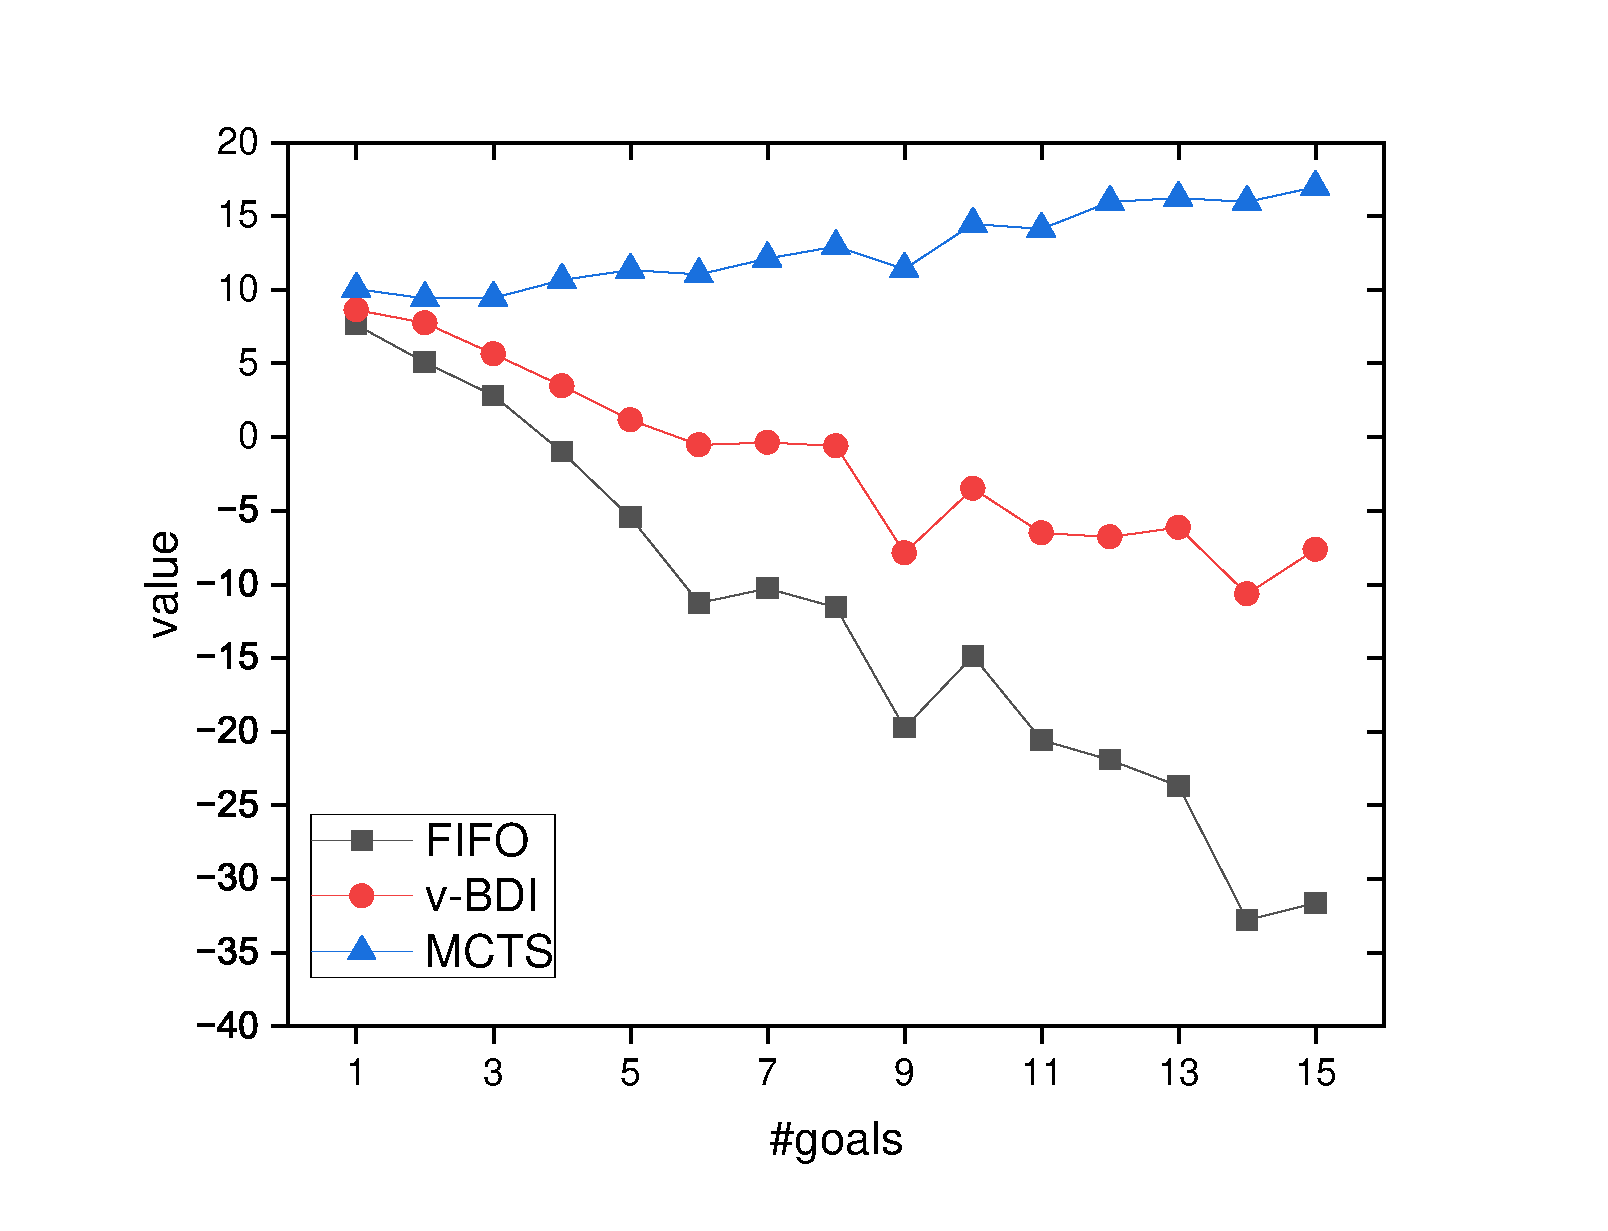
\includegraphics[scale=0.18]{goalsX_valueY_fixNorms10.pdf}
  \captionsetup{justification=centering}
  \caption{Utility}
  \label{fig:goalsX_valueY_fixNorms10}
\end{subfigure}

\begin{subfigure}{.47\textwidth}
  \centering
  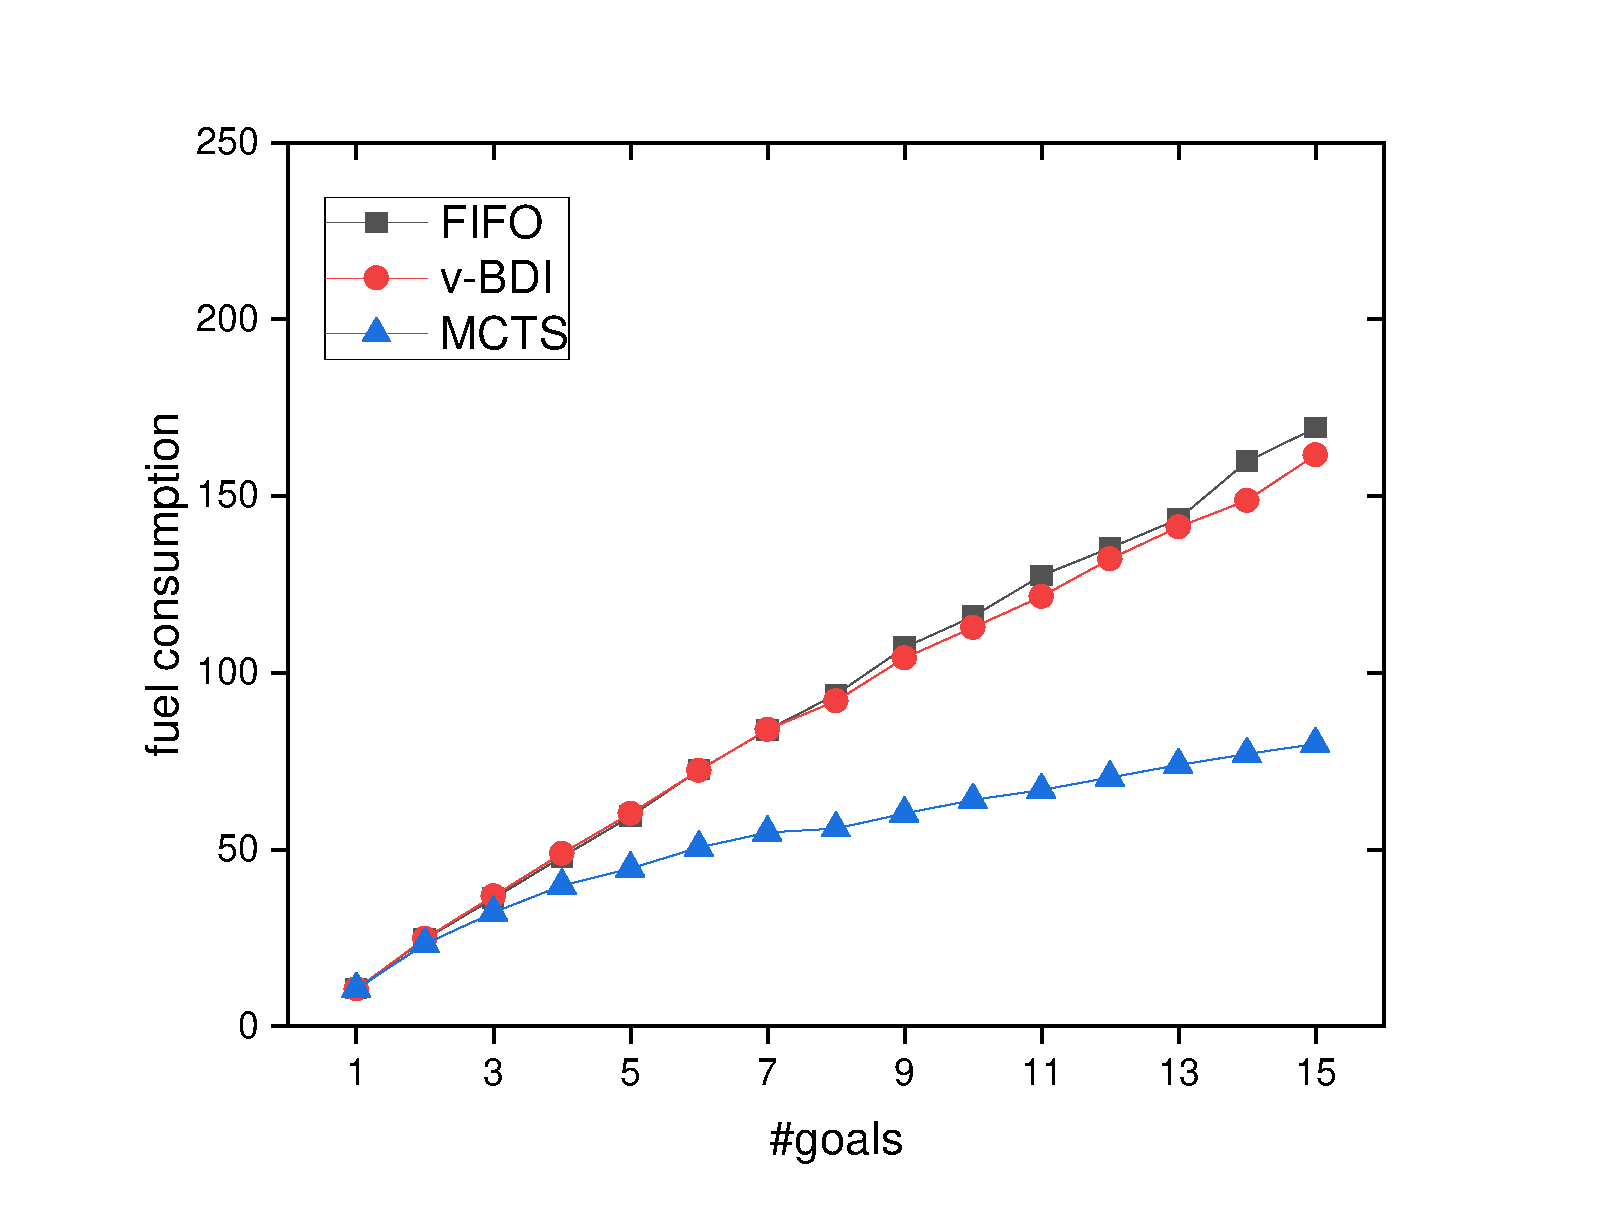
\includegraphics[scale=0.18]{goalsX_consumptionY_fixNorms10.pdf}
  \captionsetup{justification=centering}
  \caption{Fuel consumption}
  \label{fig:goalsX_consumptionY_fixNorms10}
\end{subfigure}
\begin{subfigure}{.47\textwidth}
  \centering
  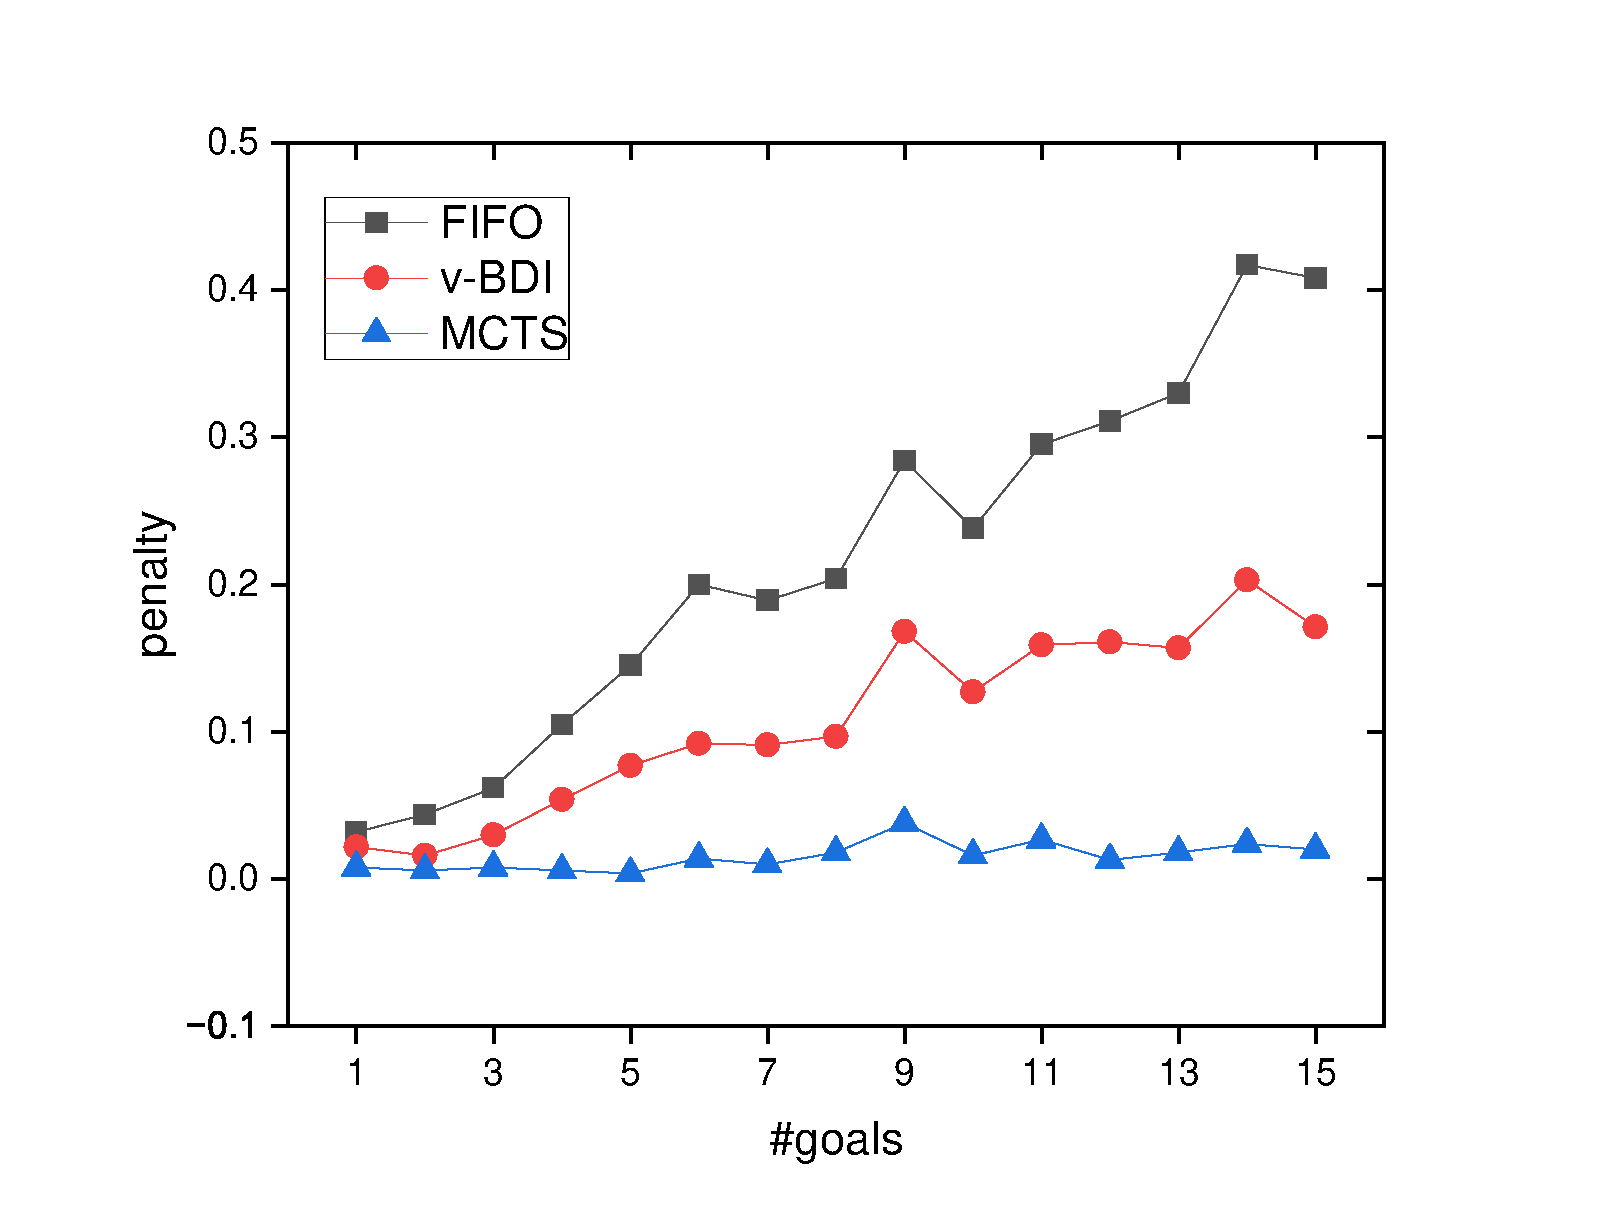
\includegraphics[scale=0.18]{goalsX_penaltyY_fixNorms10.pdf}
  \captionsetup{justification=centering}
  \caption{Penalty}
  \label{fig:goalsX_penaltyY_fixNorms10}
\end{subfigure}
\captionsetup{justification=centering}
\bicaption{norm数量为10下的实验结果}{Overall utility, fuel consumption and penalty with fixed \#norms 10}
\label{fig:all_fixNorms10}
\end{figure}

\paragraph{总价值分析}
% Note fifo
从图中可知,当实现目标数量增加时,NMG与v-BDI的总价值降低。NMG在所有情况下的性能表现都最差。
% Reason
这是因为NMG不考虑norm的影响,且忽略了不同意图之间可能出现的负面影响以及协同效应,导致性能表现低下。
% v-BDI performance
v-BDI具有比NMG更好的性能表现,因为其可以评估执行计划导致违反norm的惩罚值。v-BDI始终选择效用值最高的计划执行,从而比NMG违反更少的norm,导致最终获得更高的总价值。
% MCTS performance
最后,正如图中所示,MCTS(即\SAN 算法)有相比于NMG和v-BDI有着明显的性能优势。特别是当给定目标数量多时,MCTS与其他方法直接的差异更为显著。这是因为MCTS可以在决策时考虑到norm的影响,并且高效利用不同意图间的协同效应,通过合并不同意图间的相同动作以减少执行次数。这使得智能体有更低的可能性违反norm。与NMG、v-BDI不同,当目标数量增加时,MCTS的性能甚至略有增加(在某些部分)。这是因为在norm的数量较少的情况下(10个norm),目标数量增加时,MCTS可以更好地利用意图间的协同效应,而该协同效应带来的优势克服了违反norm的次数增加带来的危害,从而产生了更高的总价值。然而在后续实验中可以看到,当norm数量较多时,违反norm的危害很难被协同效应所克服。

% Penalty and consumption
\paragraph{电量消耗分析}
% Consumption
如图\ref{fig:goalsX_consumptionY_fixNorms10}所示, 随着目标数量的增加,所有方法的电量消耗都有所增加。与NMG和v-BDI相比,MCTS消耗的电量最少。这是由于MCTS利用意图间的协同效应节省了大量执行步骤。而NMG与v-BDI在意图选择是都遵守FIFO策略,导致执行步骤更多,造成电量的浪费。
\paragraph{惩罚值分析}
% Penalty
如图\ref{fig:goalsX_penaltyY_fixNorms10}所示, v-BDI受到的惩罚值比NMG低。这是由于v-BDI在计划选择时会有意地避免违反norm的计划,导致违反norm的次数更少。最后,相比于NMG和v-BDI,MCTS有着显著的性能优势。特别是当给定目标的数量较大时,MCTS与其他两种方法的差距更明显。

\paragraph{实验二}
在第二个实验中,norm的数量被改变为30,其他实验设置参数与实验一相同。图\ref{fig:all_fixNorms30}展示了实验结果。

\begin{figure}
\centering
\begin{subfigure}{.47\textwidth}
  \centering
  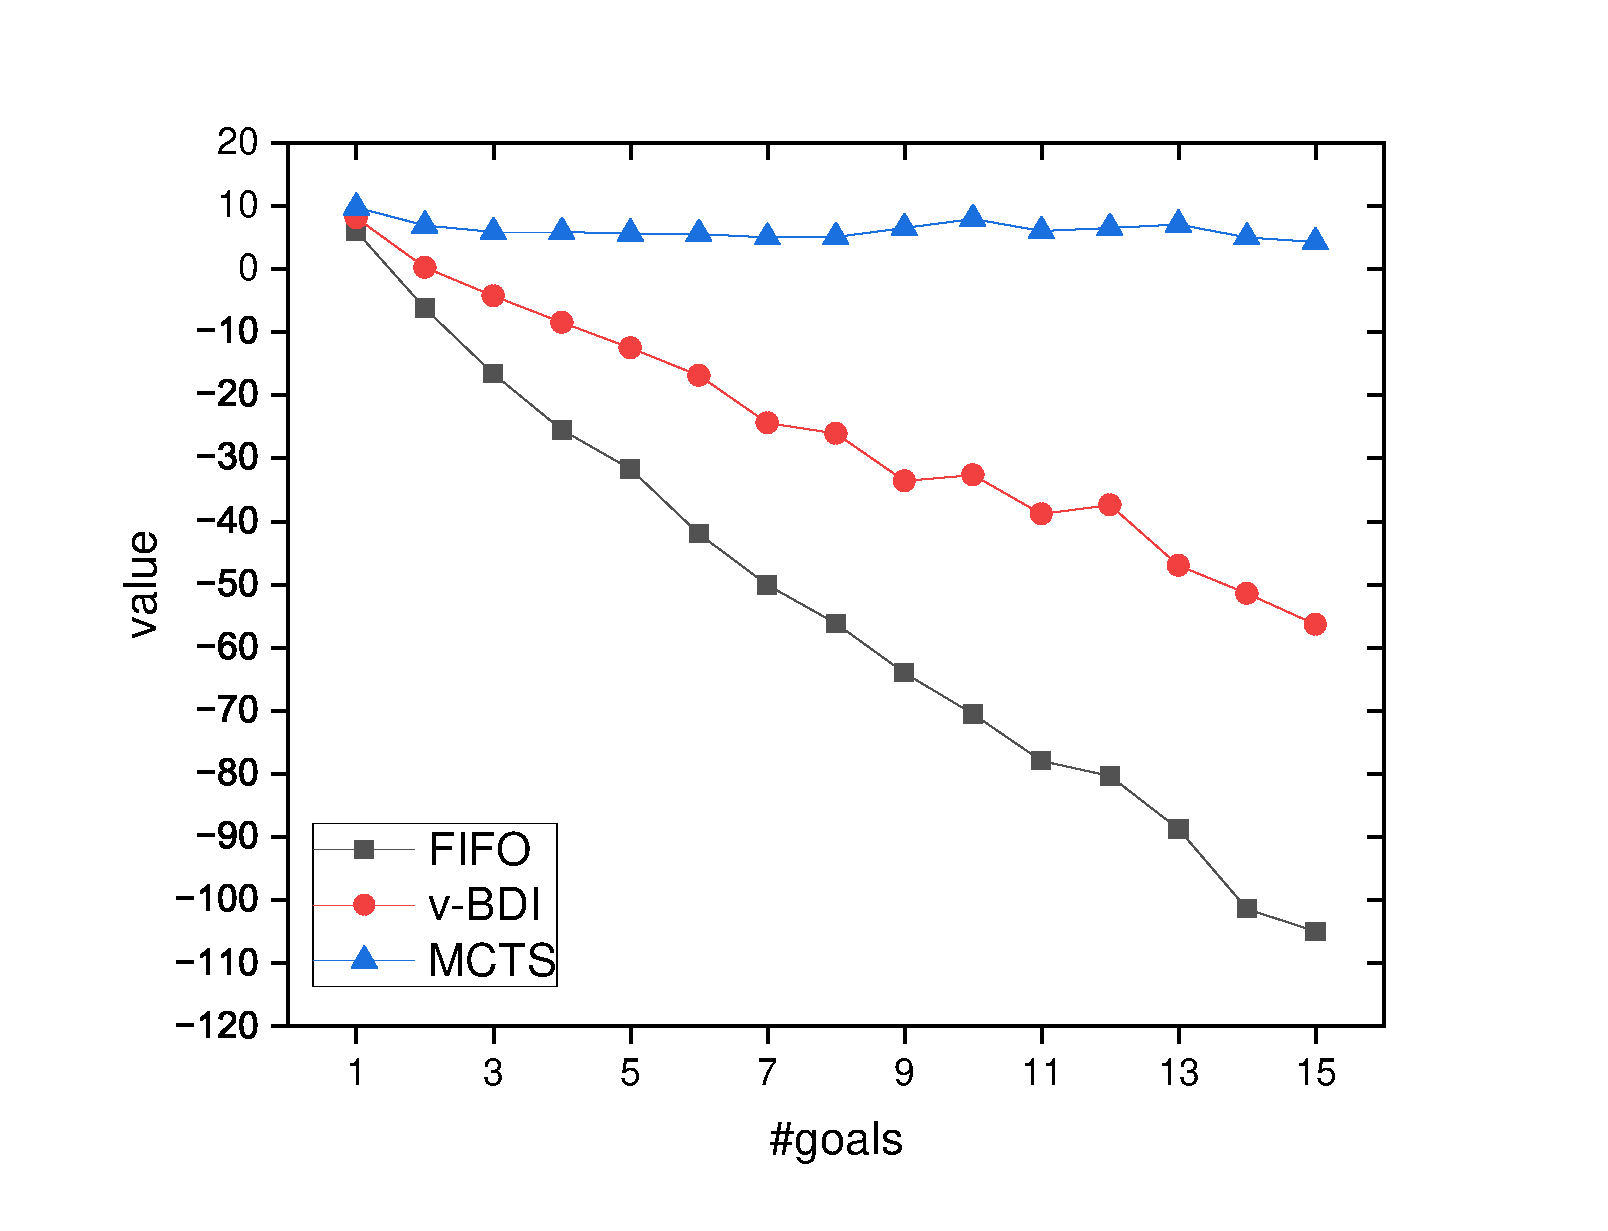
\includegraphics[scale=0.18]{goalsX_valueY_fixNorms30.pdf}
  \captionsetup{justification=centering}
  \caption{Utility}
  \label{fig:goalsX_valueY_fixNorms30}
\end{subfigure}

\begin{subfigure}{.47\textwidth}
  \centering
  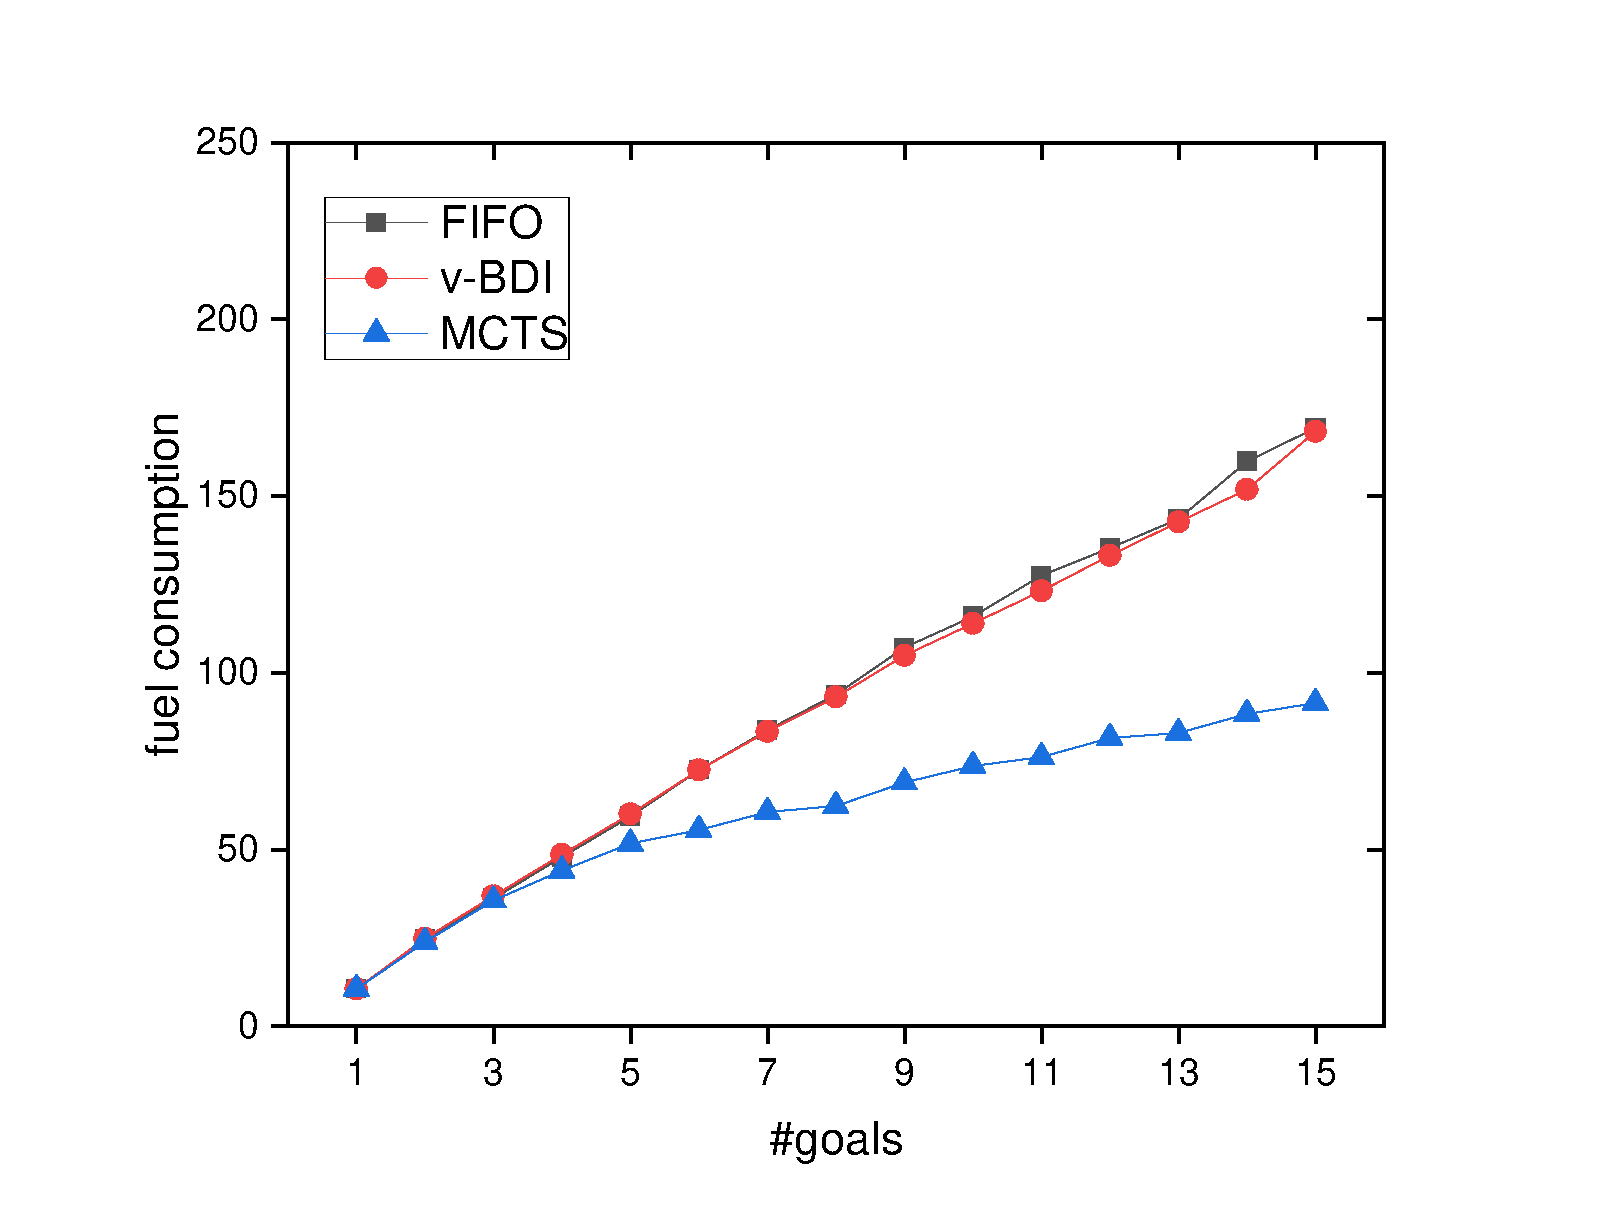
\includegraphics[scale=0.18]{goalsX_consumptionY_fixNorms30.pdf}
  \captionsetup{justification=centering}
  \caption{Fuel consumption}
  \label{fig:goalsX_consumptionY_fixNorms30}
\end{subfigure}
\begin{subfigure}{.47\textwidth}
  \centering
  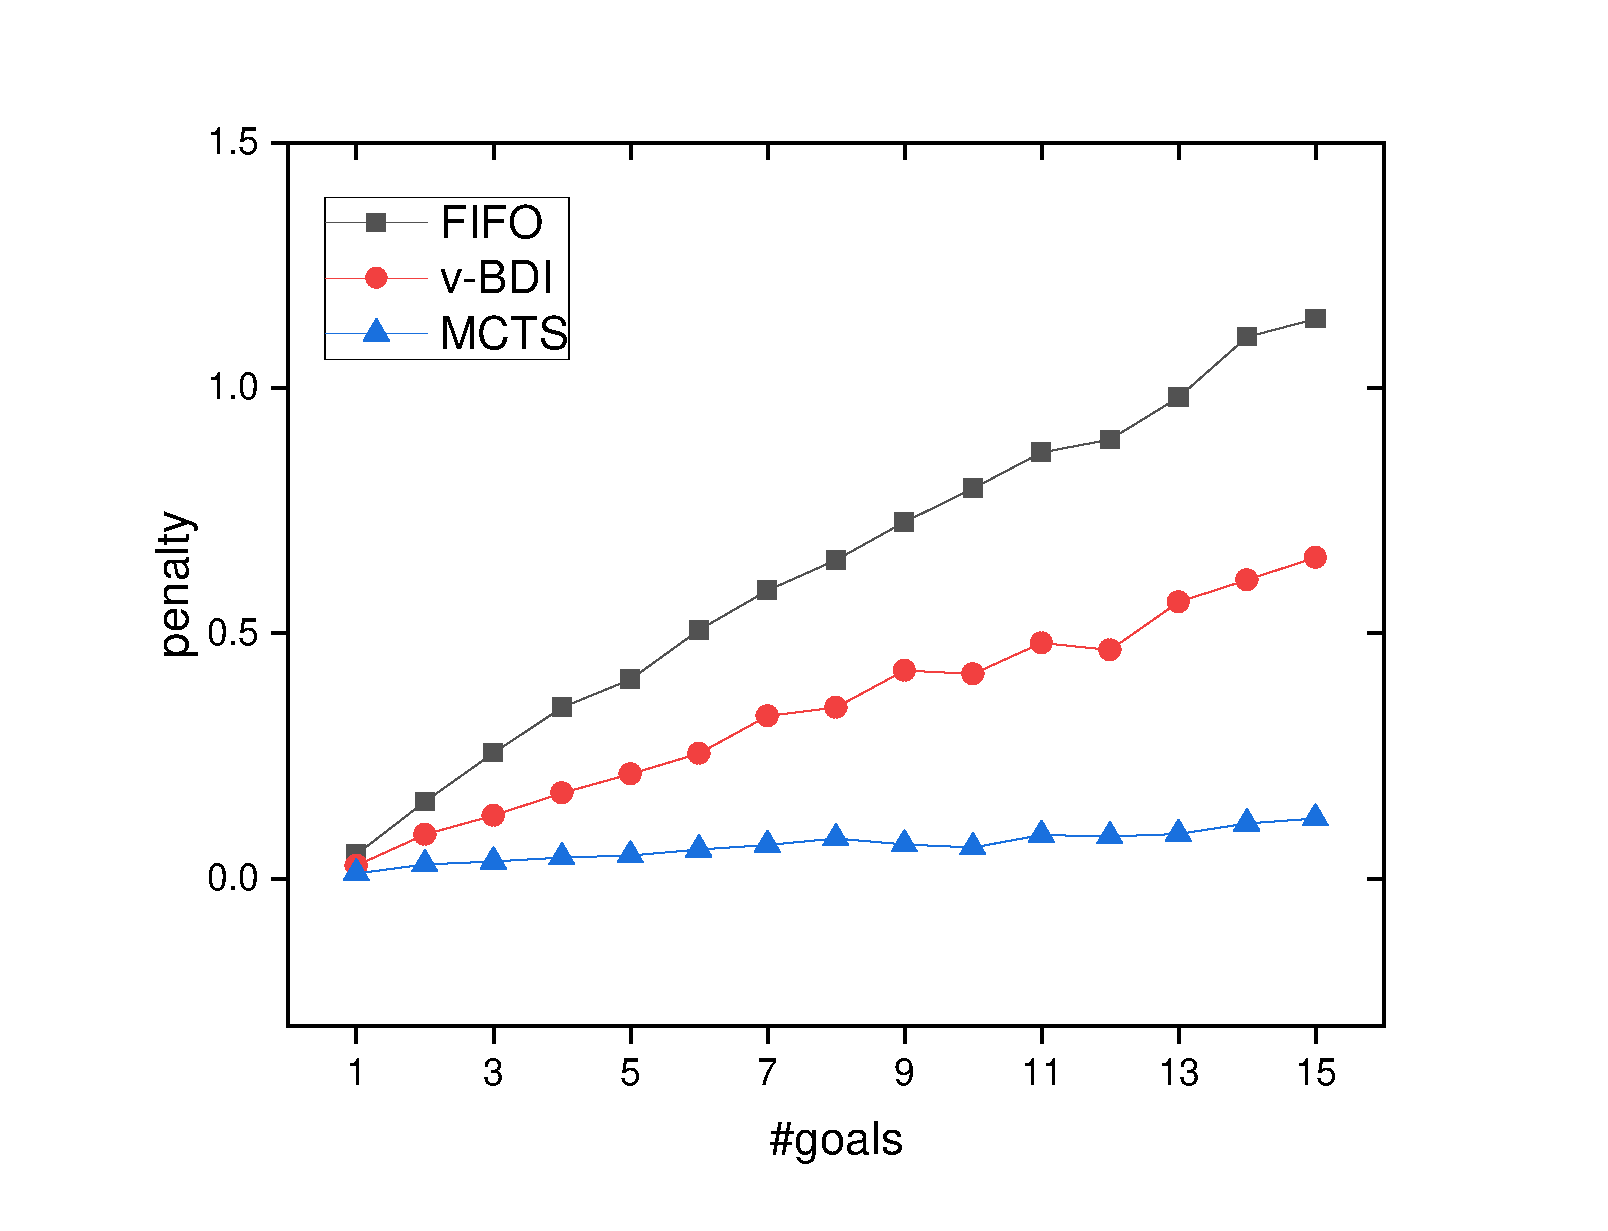
\includegraphics[scale=0.18]{goalsX_penaltyY_fixNorms30.pdf}
  \captionsetup{justification=centering}
  \caption{Penalty}
  \label{fig:goalsX_penaltyY_fixNorms30}
\end{subfigure}
\captionsetup{justification=centering}
\bicaption{norm数量为10下的实验结果}{Overall utility, fuel consumption and penalty with fixed \#norms 30}
\label{fig:all_fixNorms30}
\end{figure}

% Figure information
如图\ref{fig:goalsX_valueY_fixNorms30}所示,当实现目标数量增加时,NMG与v-BDI的性能表现明显下降。MCTS方法依然保持最高的性能表现,且几乎没有下降趋势。

% MCTS performance
然而与上一个实验相比,MCTS的性能表现有所下降。
% Reason
这是因为在当前实验中,norm的数量较多,对多目标间协同效应的利用带来的收益几乎无法抵消违反norm带来的惩罚。此外,与实验一相比,图中所示的三种方法性能表现更为稳定,这是因为当norm数量较多时,在环境中的分布更为均匀。
% Consumption
如图\ref{fig:goalsX_consumptionY_fixNorms30}所示,三种方法的电量消耗与实验一几乎相同,这是因为目标位置并没有发生变化,因此智能体需要移动的距离不会改变。
% Penalty
如图\ref{fig:goalsX_penaltyY_fixNorms30}所示, 所有方法受到的惩罚值相较于实验一都有提升。然而MCTS方法的性能表现依旧强于NMG和v-BDI。

\paragraph{实验三}
在第三个实验中,智能体被给定固定10个目标,而norm的数量从0改变至50。具体实验结果如图\ref{fig:all_fixGoals10}所示。

\begin{figure}
\centering
\begin{subfigure}{.47\textwidth}
\centering
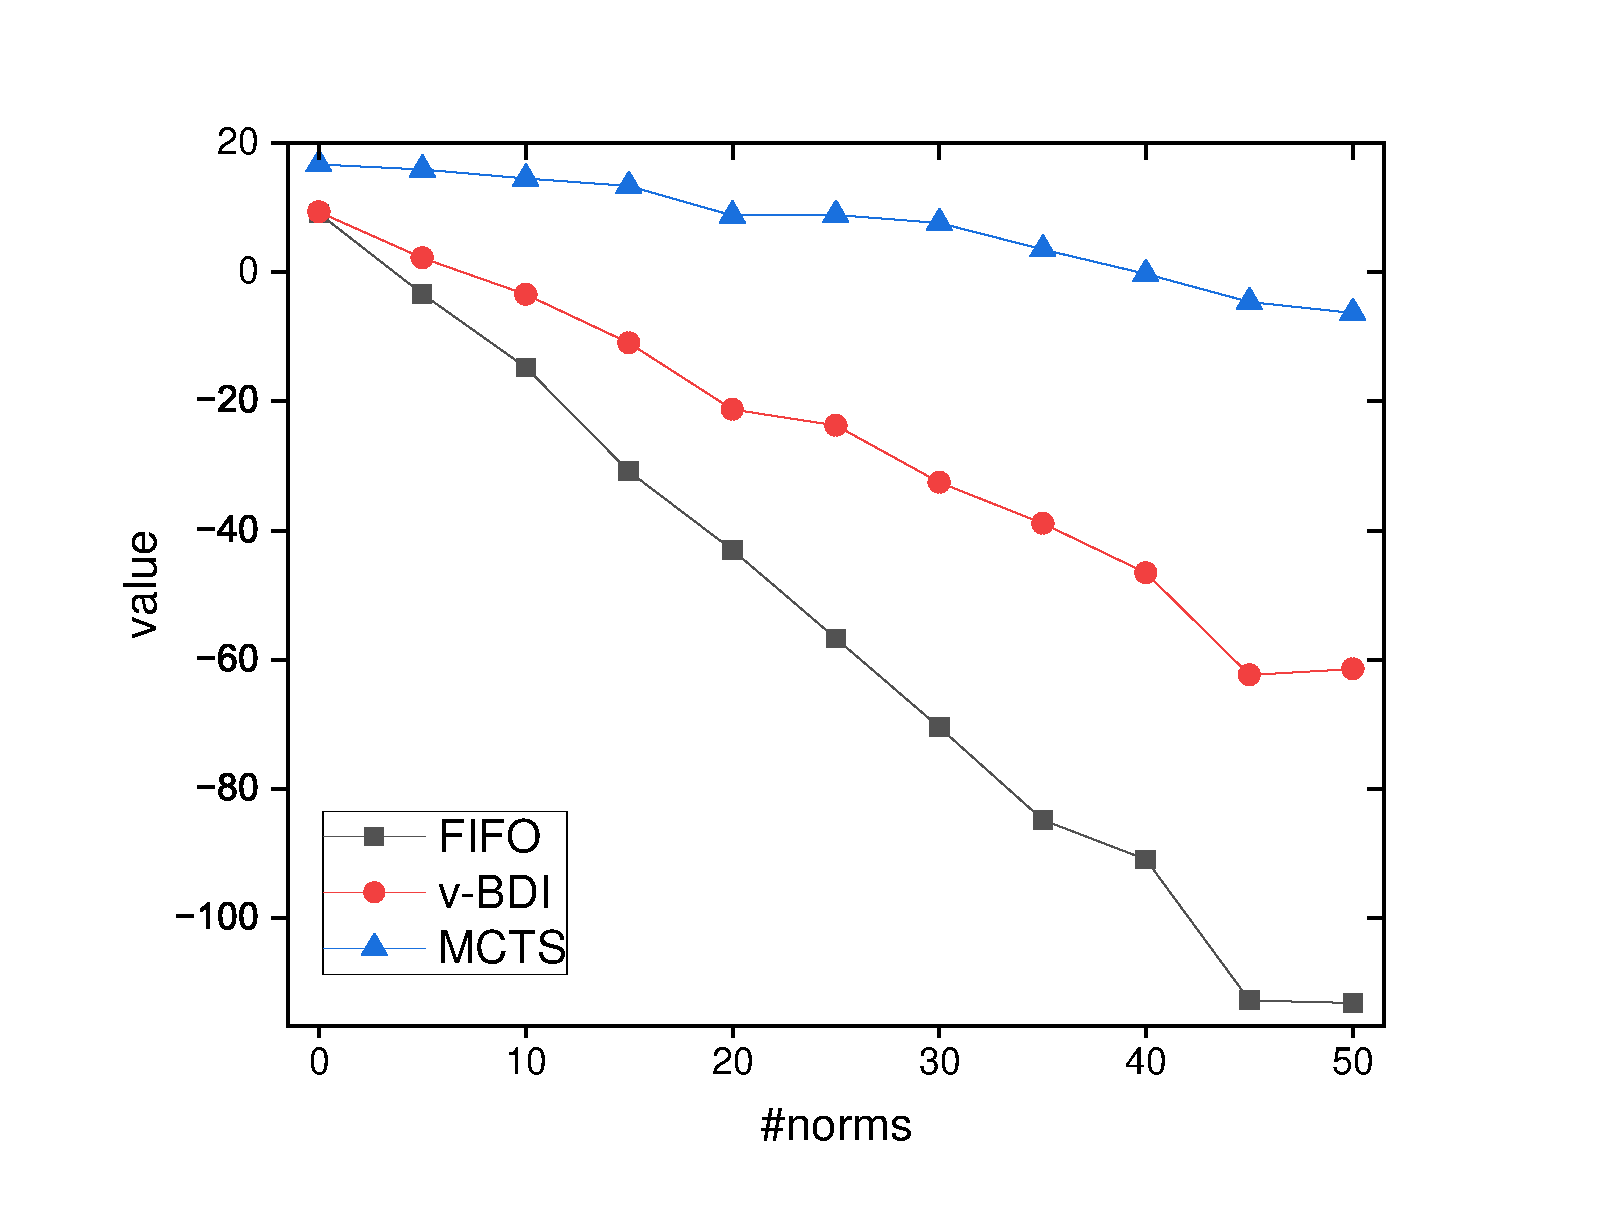
\includegraphics[scale=0.18]{normsX_valueY_fixGoals10.pdf}
\captionsetup{justification=centering}
\caption{Utility}
\label{fig:normsX_valueY_fixGoals10}
\end{subfigure}

\begin{subfigure}{.47\textwidth}
  \centering
  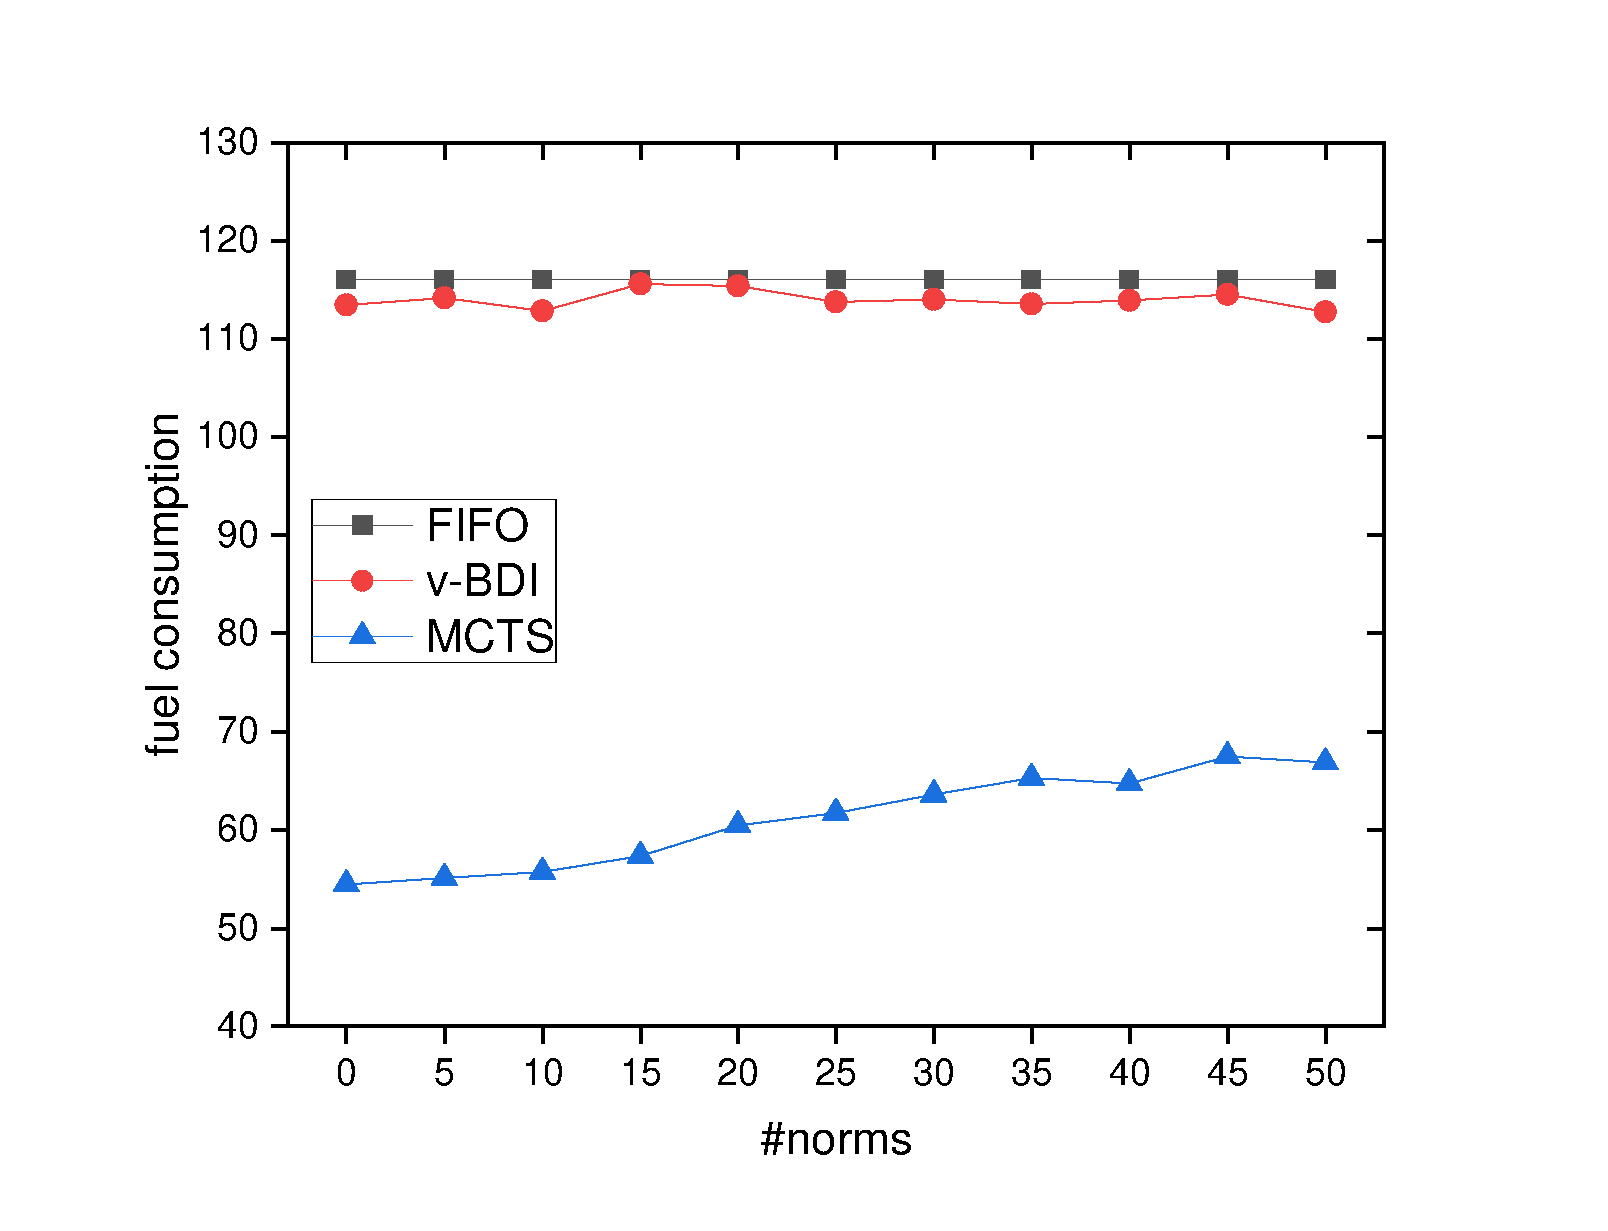
\includegraphics[scale=0.18]{normsX_consumptionY_fixGoals10.pdf}
  \captionsetup{justification=centering}
  \caption{Fuel consumption}
  \label{fig:normsX_consumptionY_fixGoals10}
\end{subfigure}
\begin{subfigure}{.47\textwidth}
  \centering
  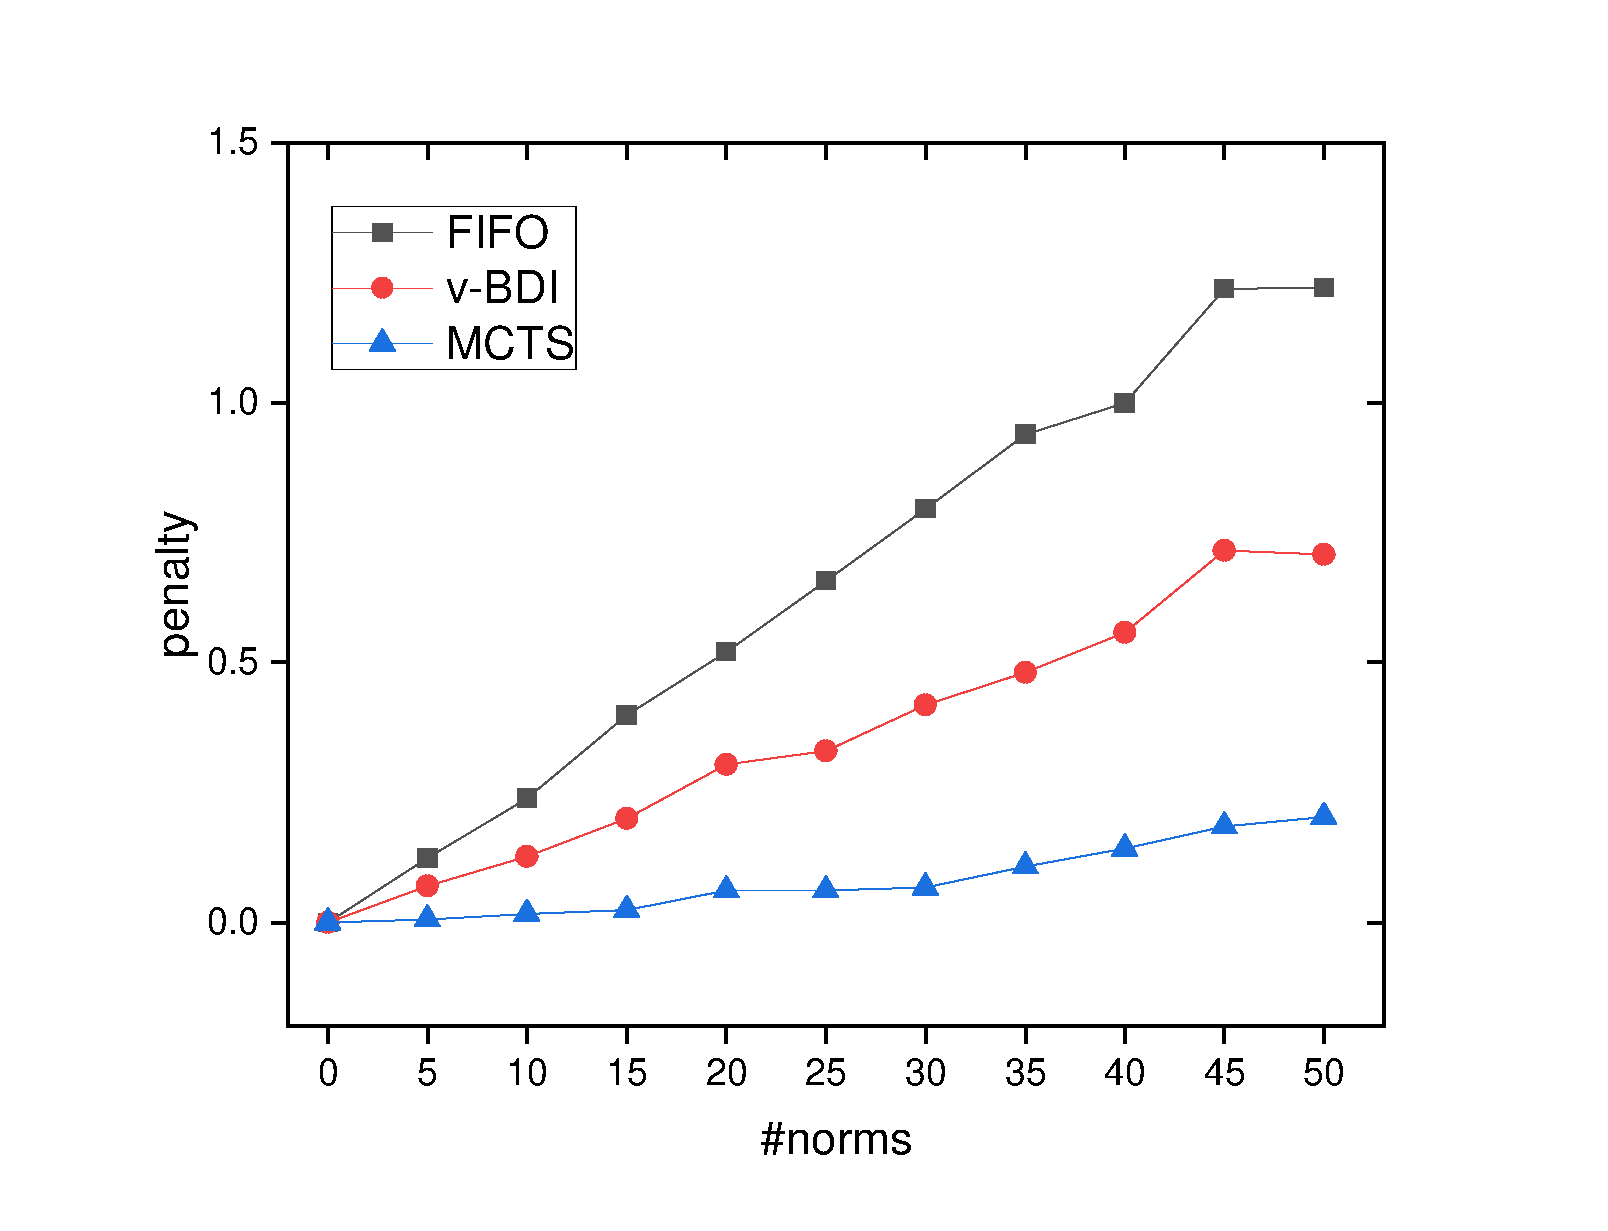
\includegraphics[scale=0.18]{normsX_penaltyY_fixGoals10.pdf}
  \captionsetup{justification=centering}
  \caption{Penalty}
  \label{fig:normsX_penaltyY_fixGoals10}
\end{subfigure}
\captionsetup{justification=centering}
\bicaption{目标数量为10下的实验结果}{Overall utility, fuel consumption and penalty with fixed \#goals 10}
\label{fig:all_fixGoals10}
\end{figure}
% Figure info
图\ref{fig:normsX_valueY_fixGoals10}展示了不同数量norm情况下每个方法的效用价值。正如所预料的,NMG的性能表现最差。
% explanation
有一个特殊情况值得注意的是当norm的数量为0时,NMG与v-BDI没有性能差异。因为当norm数量为0时,智能体是否考虑norm已经无关紧要,性能表现最终取决于实现目标的数量与电池消耗量。MCTS有着最优秀的性能表现。即使在norm的数量为0的情况下,MCTS也比NMG和v-BDI有着更好的性能表现,因为其可以利用到不同意图间的协同效应。
% Details
当norm的数量较多时,MCTS与其他方法的差距更为明显。

% Consumption
图\ref{fig:normsX_consumptionY_fixGoals10} 展示了每种方法在不同norm数量下的平均电量消耗。NMG与v-BDI消耗的电量非常相似,但是由于v-BDI的计划选择机制与NMG不同,导致与NMG相比略有波动。

% MCTS performance
在所有情况下,与NMG和v-BDI相比,MCTS消耗的电量明显更少。然而,随着norm数量的增加,MCTS的电量消耗有所增加。这是因为MCTS既重视电量消耗,也重视norm的影响。随着norm的数量增加,为了使整体收益最大化,MCTS可能会放弃一些可以利用的意图间协同效应以更好地避免违反norm的情况发生。

% Penalty
图\ref{fig:normsX_penaltyY_fixGoals10}展示了不同norm数量下各方法的平均受惩罚值。可以看出,NMG总是受到最多的惩罚值,而MCTS受到的惩罚值则比其他两种方法低很多。当norm数量较大时,不同方法收惩罚值的差异更为明显。当norm的数量为50时,MCTS仅仅受到0.2的惩罚值,而v-BDI几乎是MCTS的3倍,NMG几乎是MCTS的6倍。

\subsection{动态环境实验}
为了探究不同方法在动态环境下的性能表现,以下实验假定并非所有目标都在初始时给定。相反,一些目标会在运行时分配给智能体。
%
本实验使用变量$n$来代表两个目标的分配时间间隔。即每隔$n$周期给智能体分配一个新的目标(假定执行一个动作对应一个周期)。

\paragraph{实验四}
和实验一类似,在该实验中norm的数量被设定为10,实现目标的数量从1改变至15。另外,$n$的值被设定为5,即每隔5个周期给智能体分配一个新的目标。
\begin{figure}
\centering
\begin{subfigure}{.47\textwidth}
  \centering
  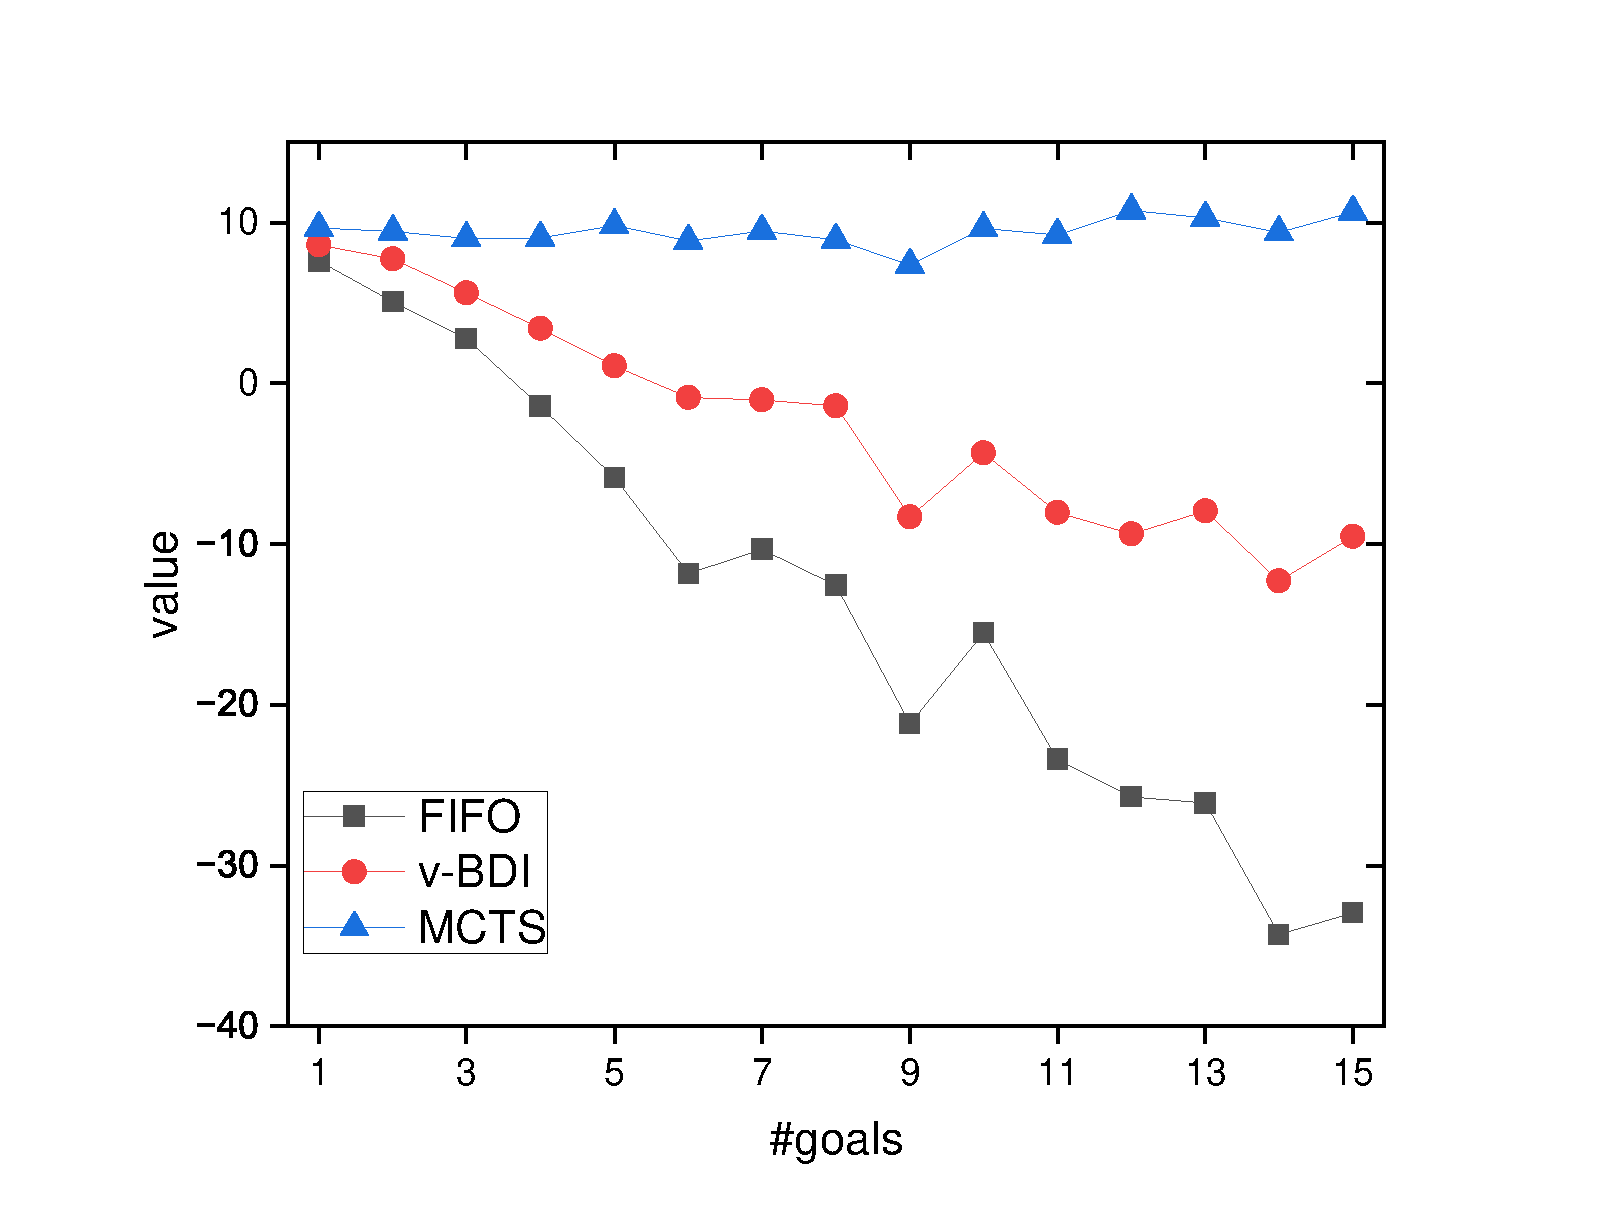
\includegraphics[scale=0.18]{goalsX_valueY_fixNorms10_dynamic.pdf}
  \captionsetup{justification=centering}
  \caption{Utility}
  \label{fig:goalsX_valueY_fixNorms10_dynamic}
\end{subfigure}

\begin{subfigure}{.47\textwidth}
  \centering
  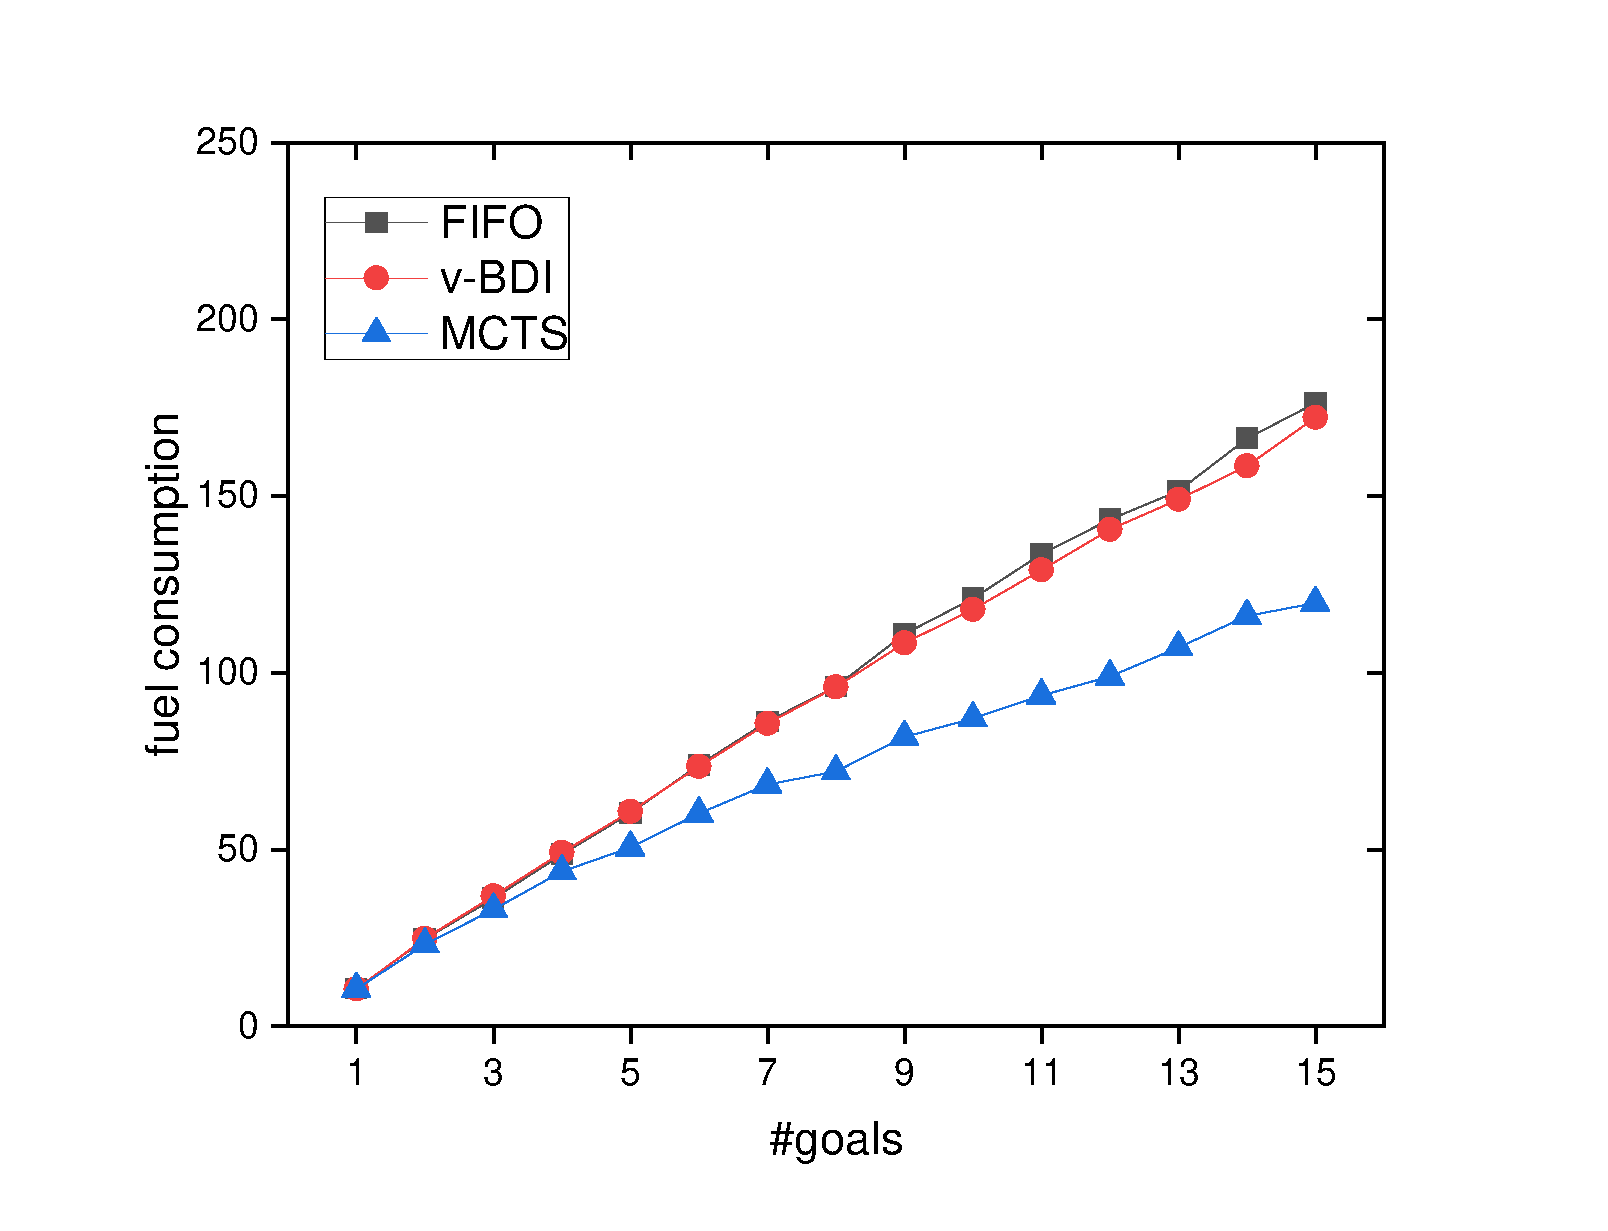
\includegraphics[scale=0.18]{goalsX_consumptionY_fixNorms10_dynamic.pdf}
  \captionsetup{justification=centering}
  \caption{Fuel consumption}
  \label{fig:goalsX_consumptionY_fixNorms10_dynamic}
\end{subfigure}
\begin{subfigure}{.47\textwidth}
  \centering
  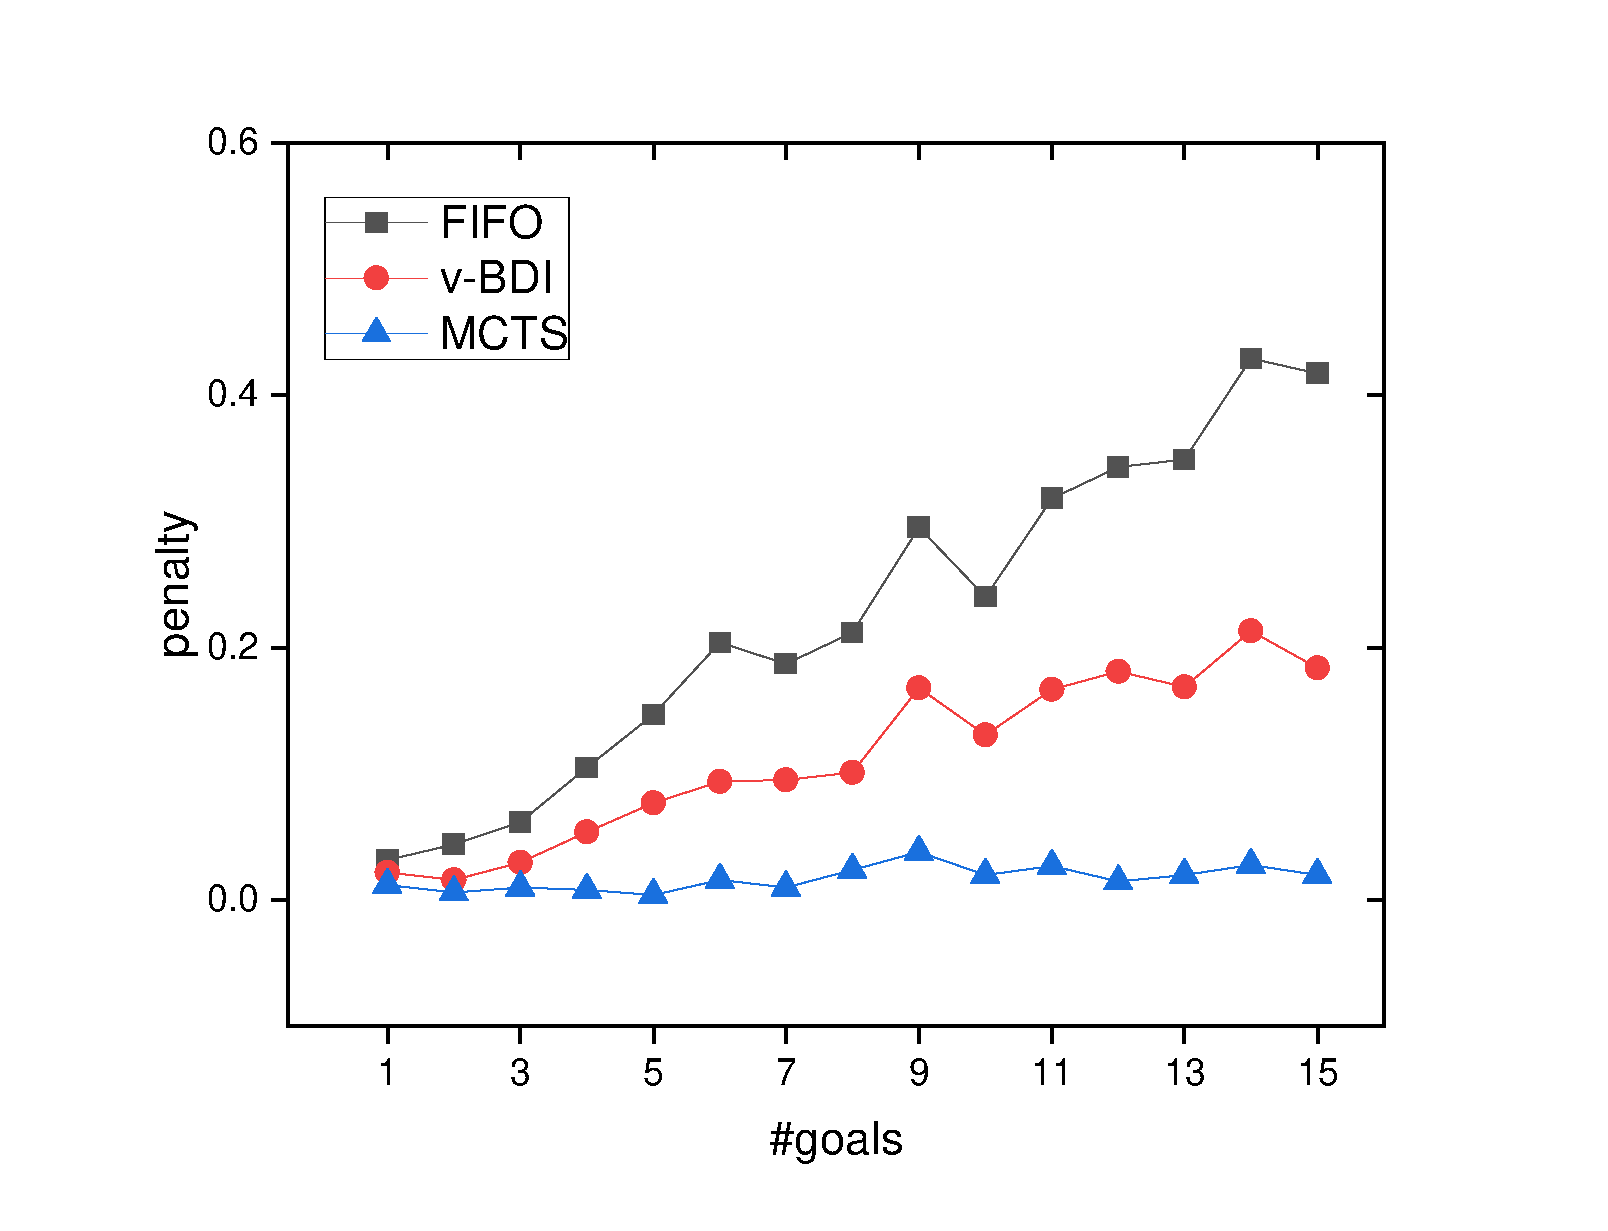
\includegraphics[scale=0.18]{goalsX_penaltyY_fixNorms10_dynamic.pdf}
  \captionsetup{justification=centering}
  \caption{Penalty}
  \label{fig:goalsX_penaltyY_fixNorms10_dynamic}
\end{subfigure}
\captionsetup{justification=centering}
\bicaption{norm数量为10下的实验结果}{Overall utility, fuel consumption and penalty with fixed \#norms 10}
\label{fig:all_fixNorms10_dynamic}
\end{figure}

图\ref{fig:goalsX_valueY_fixNorms10_dynamic}展示了每种方法的总价值。NMG和v-BDI的性能与实验一几乎相同,而MCTS则有较为明显的性能下降。这是因为即使目标在不同时间被分配给智能体,也不会影响NMG和v-BDI实现目标的顺序。唯一的区别在于,如果所有目标都在初始给定,NMG和v-BDI有更多的机会从“意料之外”的协同效应中受益。即当一个目标位于智能体移动到某一个位置的途中时,智能体可以顺便实现途中的目标,从而达到节省执行步骤的效果,这使得电量消耗降低以及违反norm的数量降低。然而,MCTS的方法受到环境动态性的影响,并行执行的目标数量降低,而智能体无法预测未来,只能根据当前状态计算出“最佳”的决策,导致对不同意图间协同效应的利用价值降低。尽管如此,MCTS的表现依然显著优于NMG和v-BDI。

% Consumption
图\ref{fig:goalsX_consumptionY_fixNorms10_dynamic} 展示了各方法的电量消耗。NMG和v-BDI的电量消耗与实验一几乎相同,而MCTS方法由于环境的动态性导致其难以利用协同效应,使得电量消耗有所增加,但是其表现依旧优于NMG和v-BDI。

% penalty
图\ref{fig:goalsX_penaltyY_fixNorms10_dynamic}展示了各方法所受到的惩罚值。与实验一相比,每种方法所受到的惩罚值几乎没有变化(目标数量相同的情况下)。这表明当前设定下的环境动态性不足以早成显著的惩罚值差异。

\vspace{3cm}

\paragraph{实验五}
在实验五中,norm的数量被设定为30。其他实验设定与实验四相同。实验结果如图\ref{fig:all_fixNorms30_dynamic}所示。
\begin{figure}
\centering
\begin{subfigure}{.47\textwidth}
  \centering
  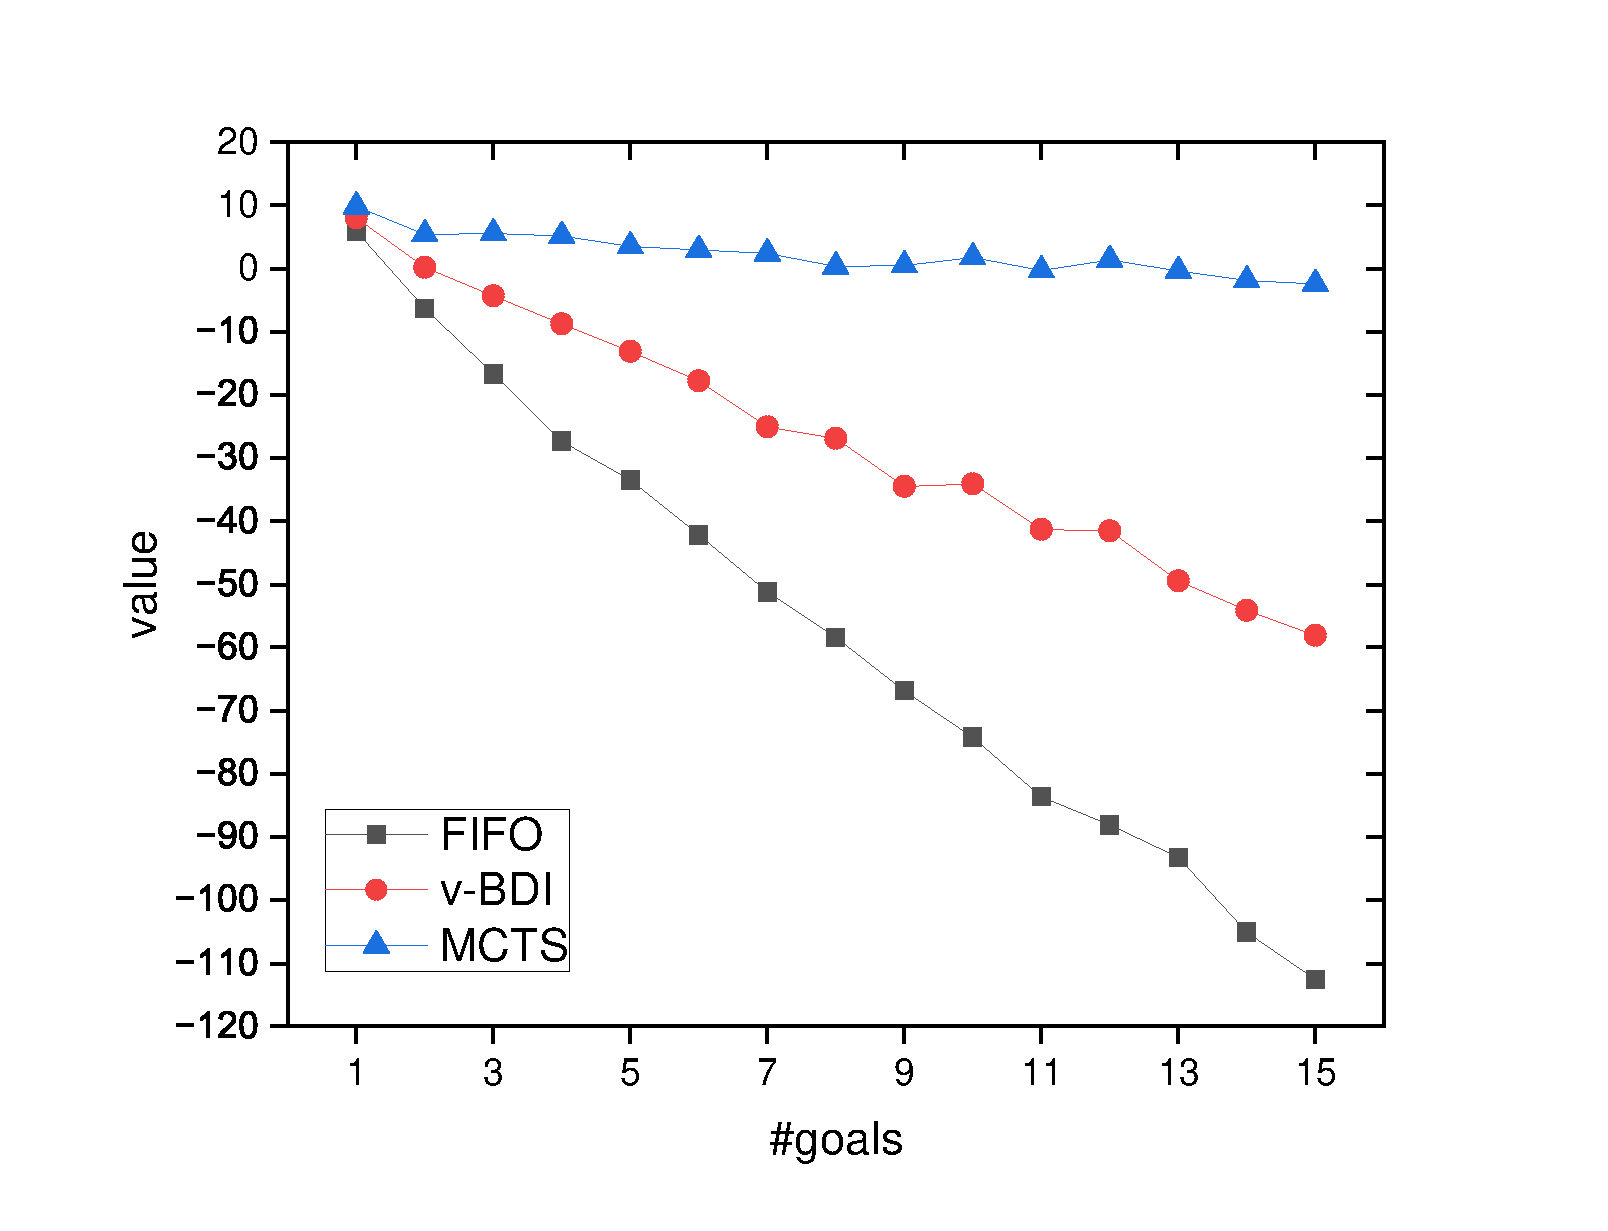
\includegraphics[scale=0.18]{goalsX_valueY_fixNorms30_dynamic.pdf}
  \captionsetup{justification=centering}
  \caption{Utility}
  \label{fig:goalsX_valueY_fixNorms30_dynamic}
\end{subfigure}

\begin{subfigure}{.47\textwidth}
  \centering
  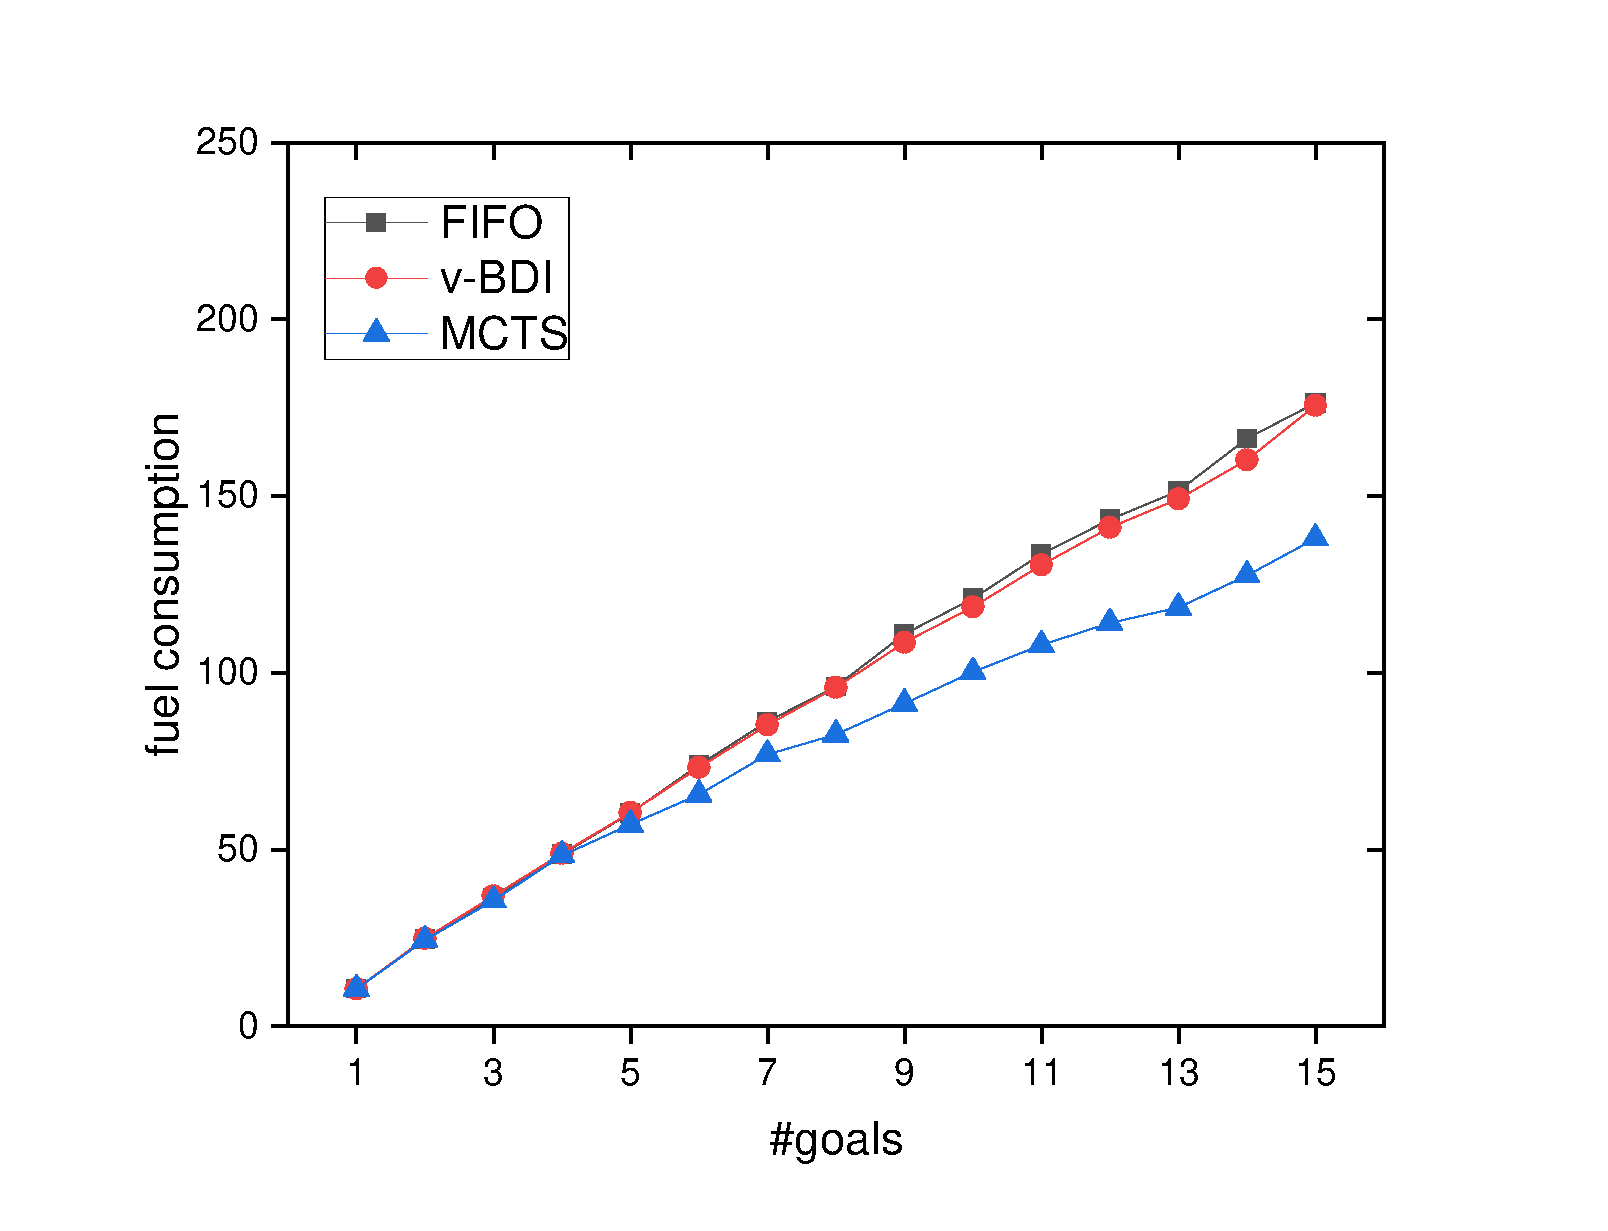
\includegraphics[scale=0.18]{goalsX_consumptionY_fixNorms30_dynamic.pdf}
  \captionsetup{justification=centering}
  \caption{Fuel consumption}
  \label{fig:goalsX_consumptionY_fixNorms30_dynamic}
\end{subfigure}
\begin{subfigure}{.47\textwidth}
  \centering
  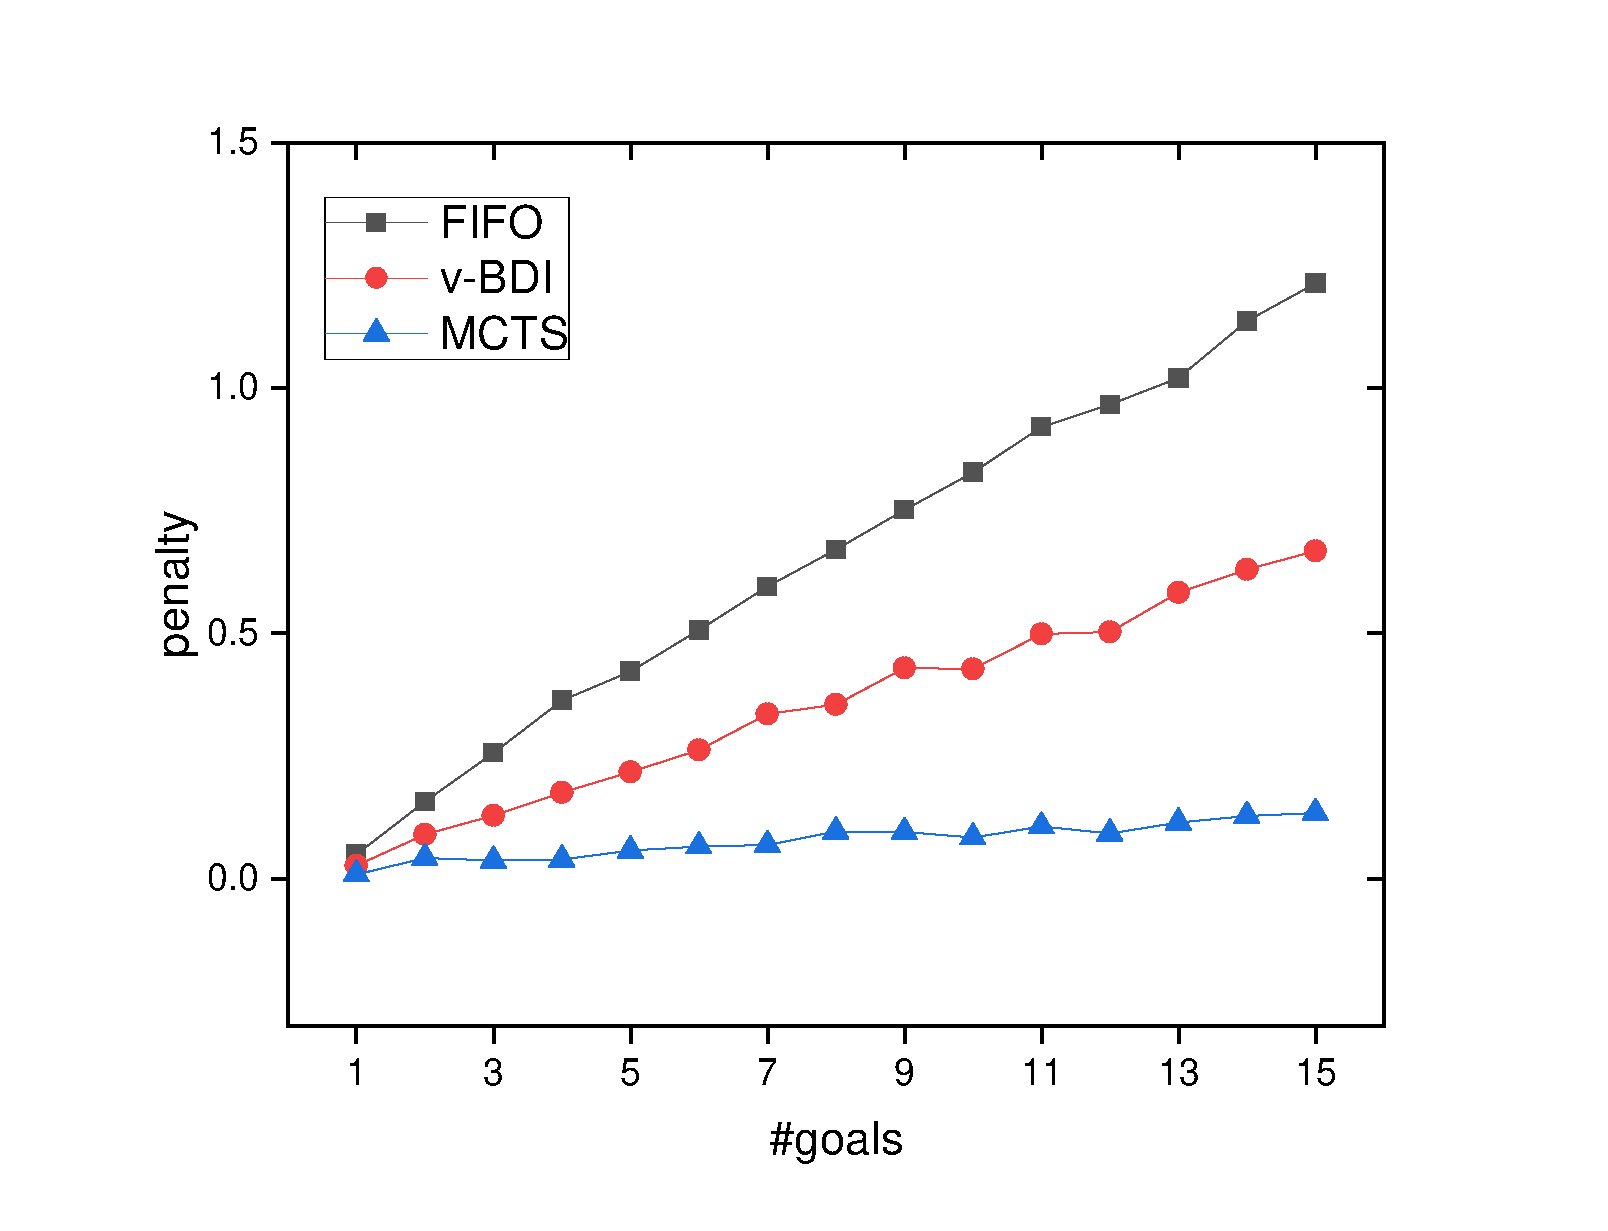
\includegraphics[scale=0.18]{goalsX_penaltyY_fixNorms30_dynamic.pdf}
  \captionsetup{justification=centering}
  \caption{Penalty}
  \label{fig:goalsX_penaltyY_fixNorms30_dynamic}
\end{subfigure}
\captionsetup{justification=centering}
\bicaption{norm数量为30下的实验结果}{Overall utility, fuel consumption and penalty with fixed \#norms 30}
\label{fig:all_fixNorms30_dynamic}
\end{figure}

该设定下的实验结果与实验二非常类似。相比于NMG和v-BDI,MCTS有着显著的性能优势。v-BDI比NMG的性能表现更好,但是仍然无法与MCTS相比较。特别是当实现目标数量较大时,MCTS的性能优势尤为明显。

\paragraph{实验六}
在实验六中,智能体实现目标的数量被固定为10,norm的数量被固定为30。分配目标的时间间隔$n$从1改变至15。具体实验结果如图\ref{fig:all_fixGoals10Norms30}所示。

\begin{figure}
\centering
\begin{subfigure}{.47\textwidth}
\centering
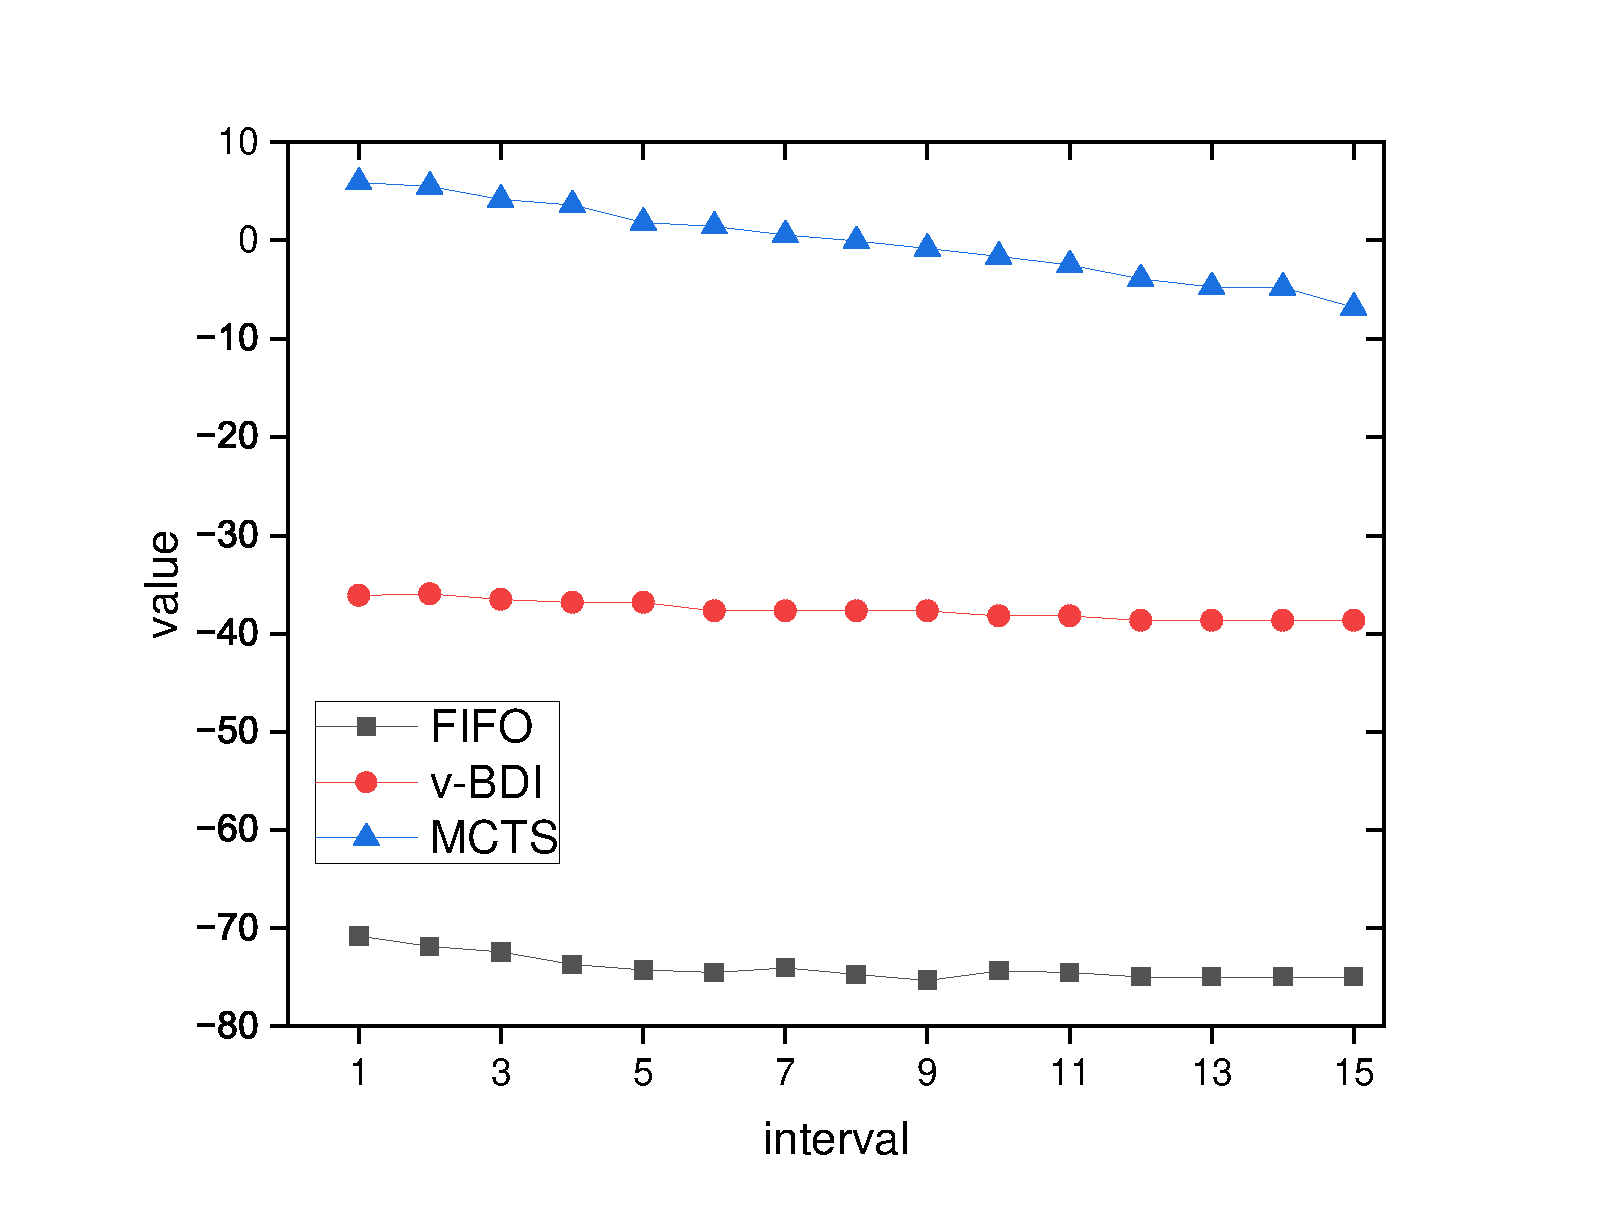
\includegraphics[scale=0.18]{intervalX_valueY_fixGoals10.pdf}
\captionsetup{justification=centering}
\caption{Overall utility}
\label{fig:intervalX_valueY_fixGoals10}
\end{subfigure}

\begin{subfigure}{.47\textwidth}
  \centering
  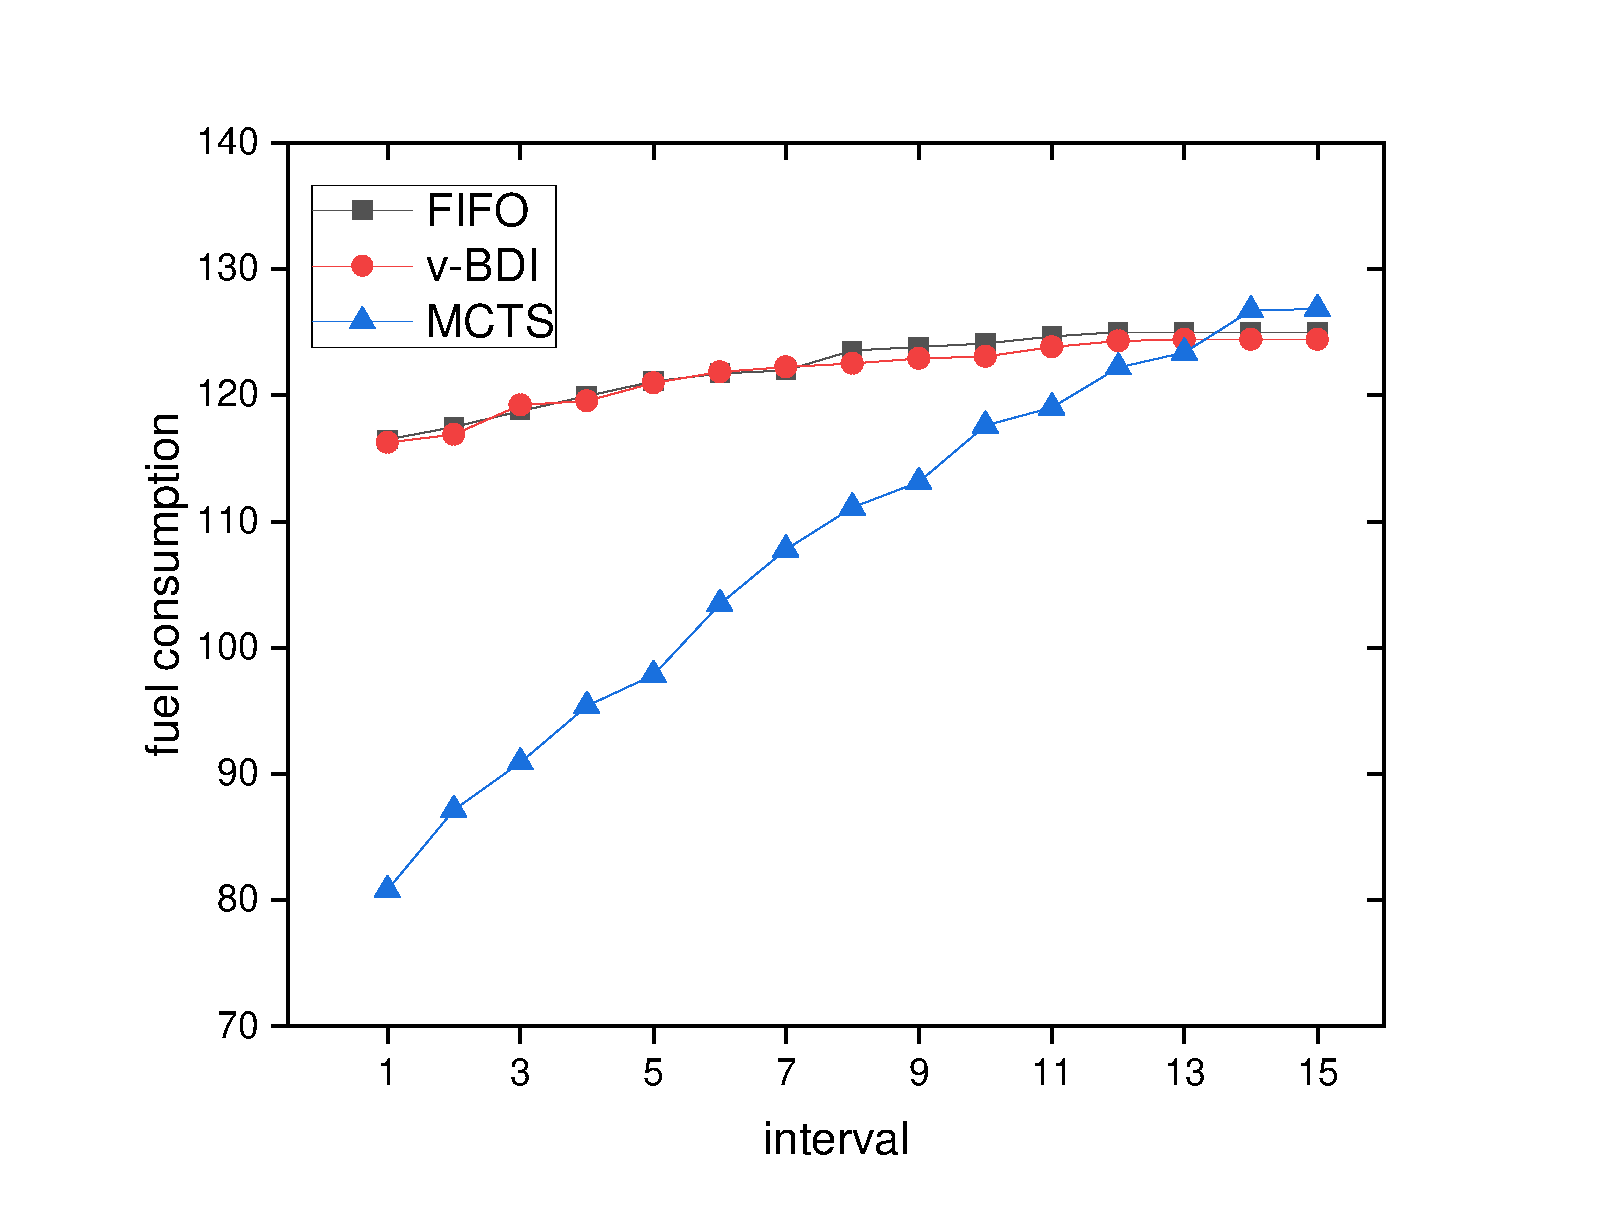
\includegraphics[scale=0.18]{intervalX_consumptionY_fixGoals10.pdf}
  \captionsetup{justification=centering}
  \caption{Fuel consumption}
  \label{fig:intervalX_consumptionY_fixGoals10}
\end{subfigure}
\begin{subfigure}{.47\textwidth}
  \centering
  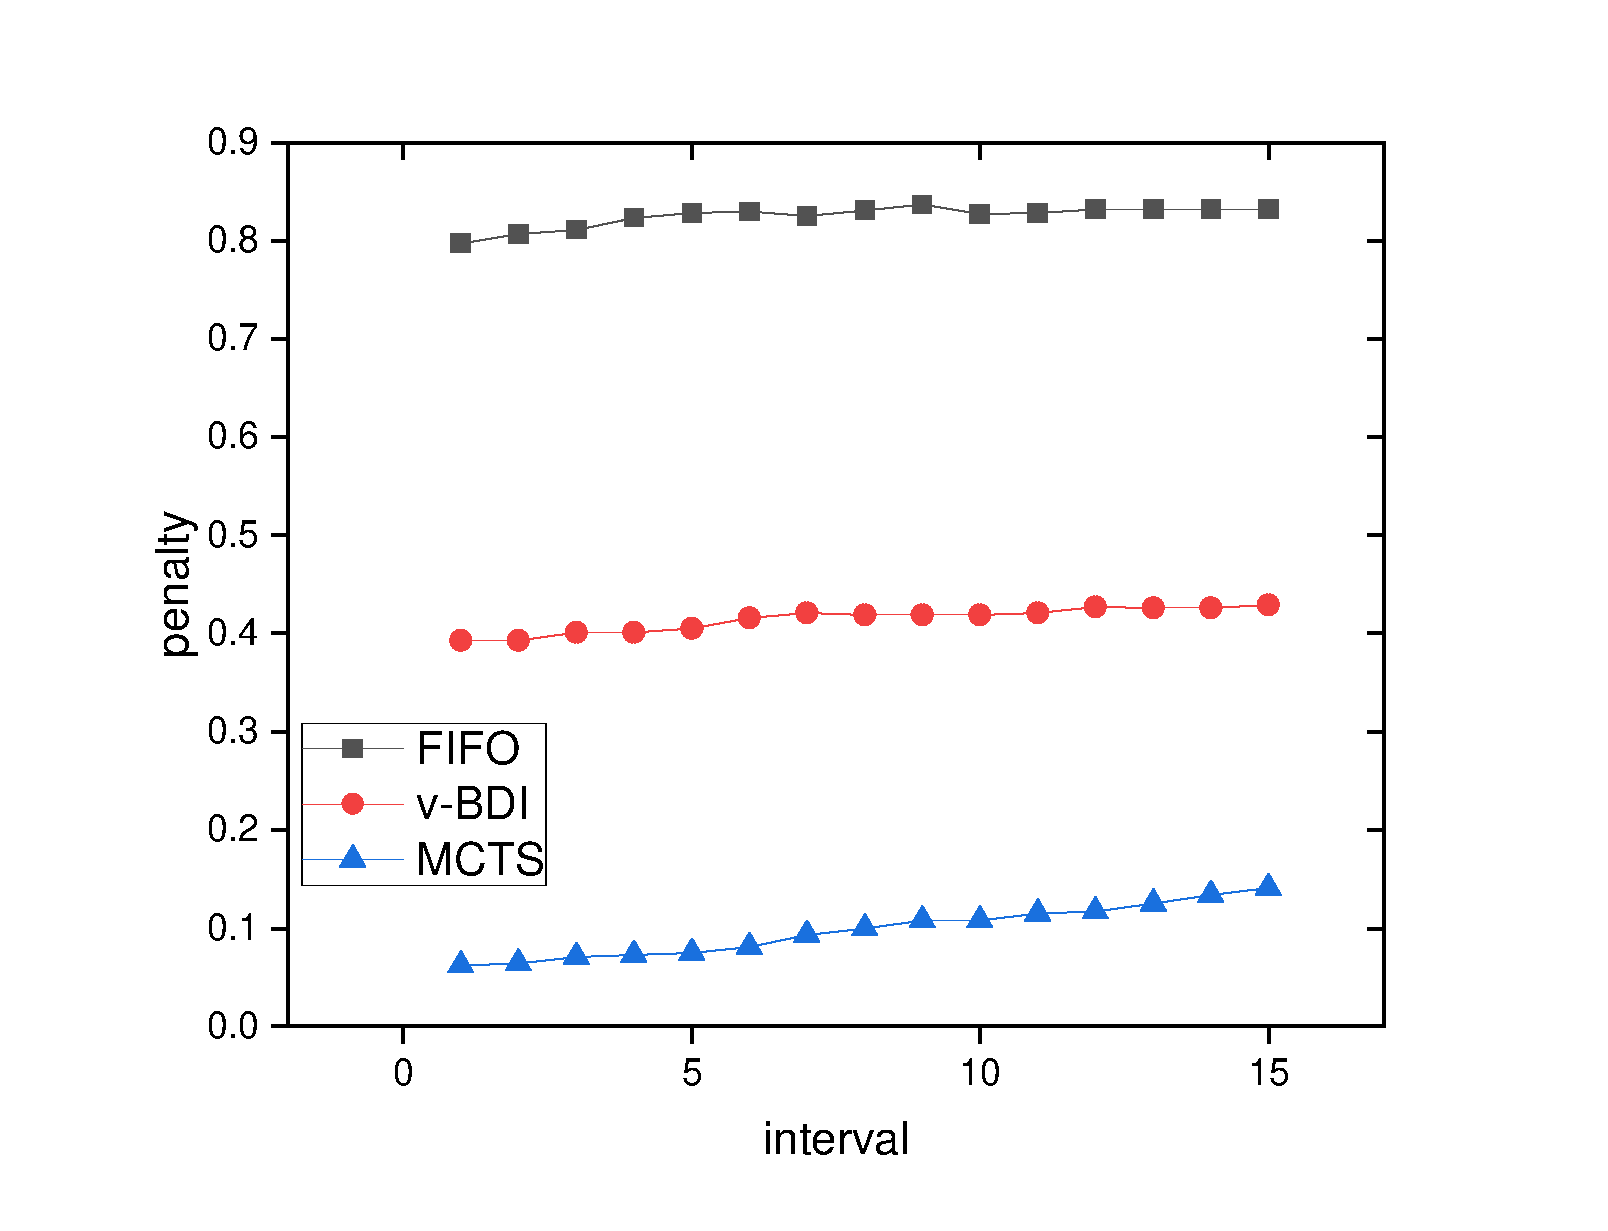
\includegraphics[scale=0.18]{intervalX_penaltyY_fixGoals10.pdf}
  \captionsetup{justification=centering}
  \caption{Penalty}
  \label{fig:intervalX_penaltyY_fixGoals10}
\end{subfigure}
\captionsetup{justification=centering}
\bicaption{目标数量为10且norm数量为30下的实验结果}{Overall utility, fuel consumption and penalty with fixed \#goals 10 and \#norms 30}
\label{fig:all_fixGoals10Norms30}
\end{figure}
% Figure information
如图\ref{fig:intervalX_valueY_fixGoals10}所示,MCTS方法依旧优于NMG和v-BDI。然而,MCTS方法的收益随着时间间隔的增加而有所减少。
% Reason
当$n$较小时,有更多的并行目标,因此智能体可以更多地利用多意图间的协同效应。当$n$设定为15时,智能体几乎无法从协同效应中受益,因为这种情况下大多数时候智能体只有一个目标。然而,MCTS仍然比v-BDI表现更为优秀,因为MCTS可以更好地对norm进行决策推理并利用多意图间协同效应,从而减少移动量以及违反norm的次数。

% Consumption
图\ref{fig:intervalX_consumptionY_fixGoals10}展示了不同时间间隔下各方法的平均耗电量。所有方法的耗电量都随着时间间隔的变大而增加。然而,值得注意的是,与NMG和v-BDI相比,MCTS的电量消耗增长更为明显。当$n$大于13时,其电量消耗甚至大于NMG和v-BDI。
% Explanation
这是因为MCTS主要考虑的是整体效用值,这导致其放弃了一些原本可以利用的意图间协同效应而避免违反norm,已获得更高的整体收益。
% penalty
图\ref{fig:intervalX_penaltyY_fixGoals10}展示了每种方法在不同时间间隔下单平均惩罚值。与NMG相比,v-BDI收到的惩罚值更少。由于固定的实现目标顺序,这两种方法的惩罚值几乎不会随着时间间隔的增加而改变。然而,相比之下MCTS所受惩罚值非常低。另外,由于NCMTS总是基于当前环境进行决策,导致随着$n$的增加,MCTS所执行步骤数量增加,最终使得智能体违反更多的norm,受到的惩罚值有明显的增加。
\section{本章总结}
本章提出了一种基于\SA 的意图调度算法\SAN 。\SAN 可以在norm约束下对智能体进行意图调度。另外,基于火星探测器的模拟场景,本章在静态环境以及动态环境下对\SAN 的性能进行了分析。实验结果表明\SAN 与其他方法(NMG和v-BDI)相比有着显著的性能优势。即使在norm的数量非常多时,\SAN 仍然可以可靠地地避免对norm
的违反同时高效利用多个并发意图之间的协同效应,最终得到较高的整体价值收益。

本文的下一章将考虑如何基于时序逻辑(Linear Temporal Logic,LTL),并将其与MCTS算法有效结合,使得智能体同时处理实现型目标、维持型目标以及norm;并且提高智能体的可扩展性,允许智能体处理各种类型的用LTL表示的目标和norm。
